\documentclass[landscape,10pt]{beamer} % use larger type; default would be 10pt
\usepackage{graphicx}
\usepackage{hyperref}
\usepackage{pgf,pgffor}
%\usepackage{geometry} % SIVUN DIMENSION MUUTTAMISTA VARTEN
%\geometry{a4paper} % or letterpaper (US) or a5paper or....
%\addtolength{\topmargin}{-.5in} 
\addtolength{\topmargin}{.2cm} 
%\addtolength{\textheight}{1.75in}
%\addtolength{\oddsidemargin}{.1in}
\addtolength{\oddsidemargin}{-.3in}
%\addtolength{\evensidemargin}{-.4in}
\addtolength{\evensidemargin}{-.3in}
\addtolength{\textwidth}{0.6in}
\newcommand{\commentout}[1]{}

\pagestyle{empty}
\def\FineEtaBins{_eta00-03,_eta03-05,_eta05-08,_eta08-10,_eta10-13,_eta13-15,_eta15-17,_eta17-19,_eta19-22,_eta22-23,_eta23-25,_eta25-26,_eta26-29,_eta29-30,_eta30-31,_eta31-35,_eta35-38}%,_eta38-52}

\begin{document}

\begin{centering}
{. }\\
{. }\\
{. }\\
{. }\\
{. }\\
{. }\\
{. }\\
Z+Jet/dijet global fit status\\
\today\\
Mikko Voutilainen, Henning Kirschenmann
U. Helsinki and HIP\\
\end{centering}
\newpage

The following slides use inputs from the L3Res team, posted on the (JEC agenda of Wednesday 26 Jul 2017 ( \url{https://indico.cern.ch/event/656050/contributions/2672547/attachments/1499094/2369817/JEC_combinations_2017-09-04.tar.gz} ) beginning of September.\\
For dijets, the 10July and 12July input files are taken from JEC agenda 5 Jul 2017 \url{https://indico.cern.ch/event/651009/}. The wide bin results (10 July) and the fine bin results (12 July) are merged in order to get a eta 0-1.3 fir as well.\\
The inputs have been processed on top of the \verb|Summer16_03Feb2017H_V3_[DATA/MC]| corrections in the JEC database (shown as reference).\\
%.\\

\newpage
%  \n \\
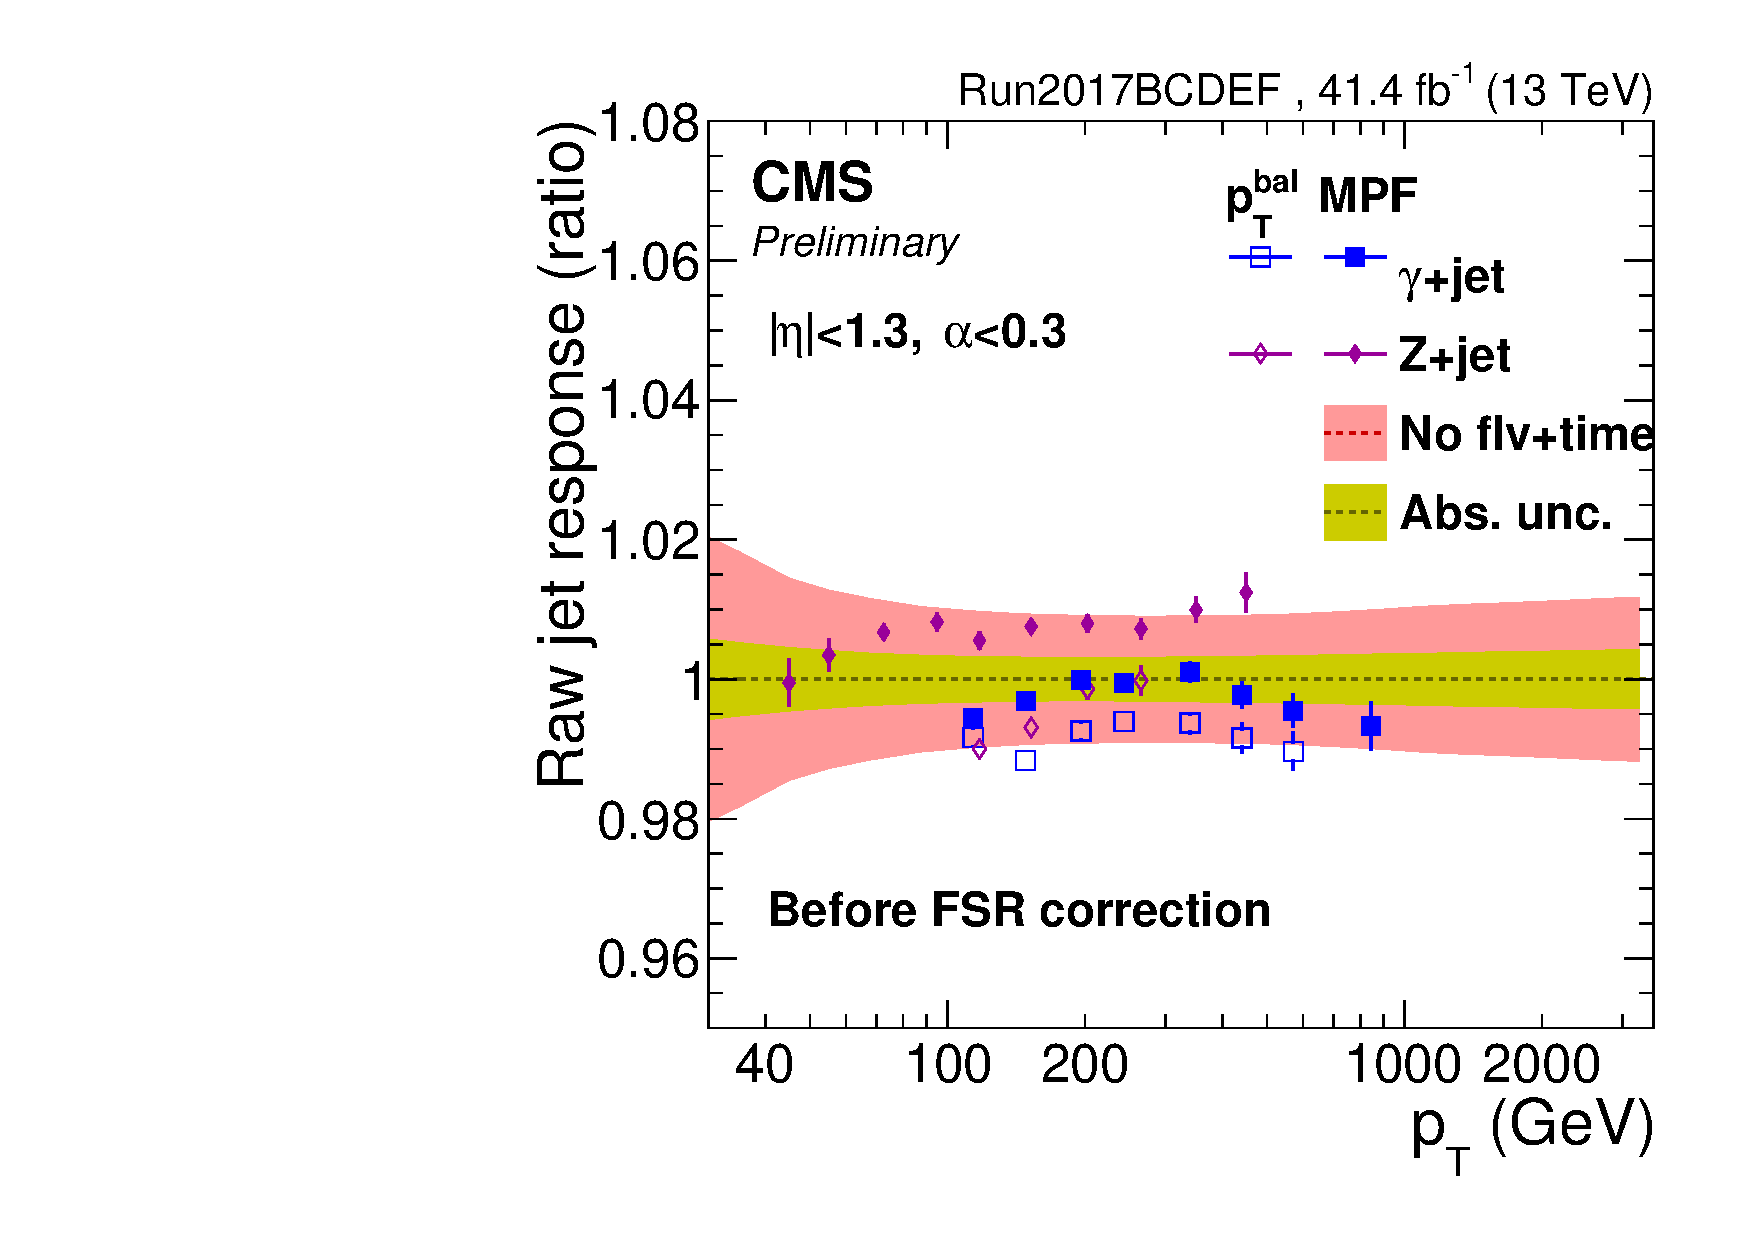
\includegraphics[width=0.32\textwidth]{BCDEFGH/globalFitL3res_raw.pdf}
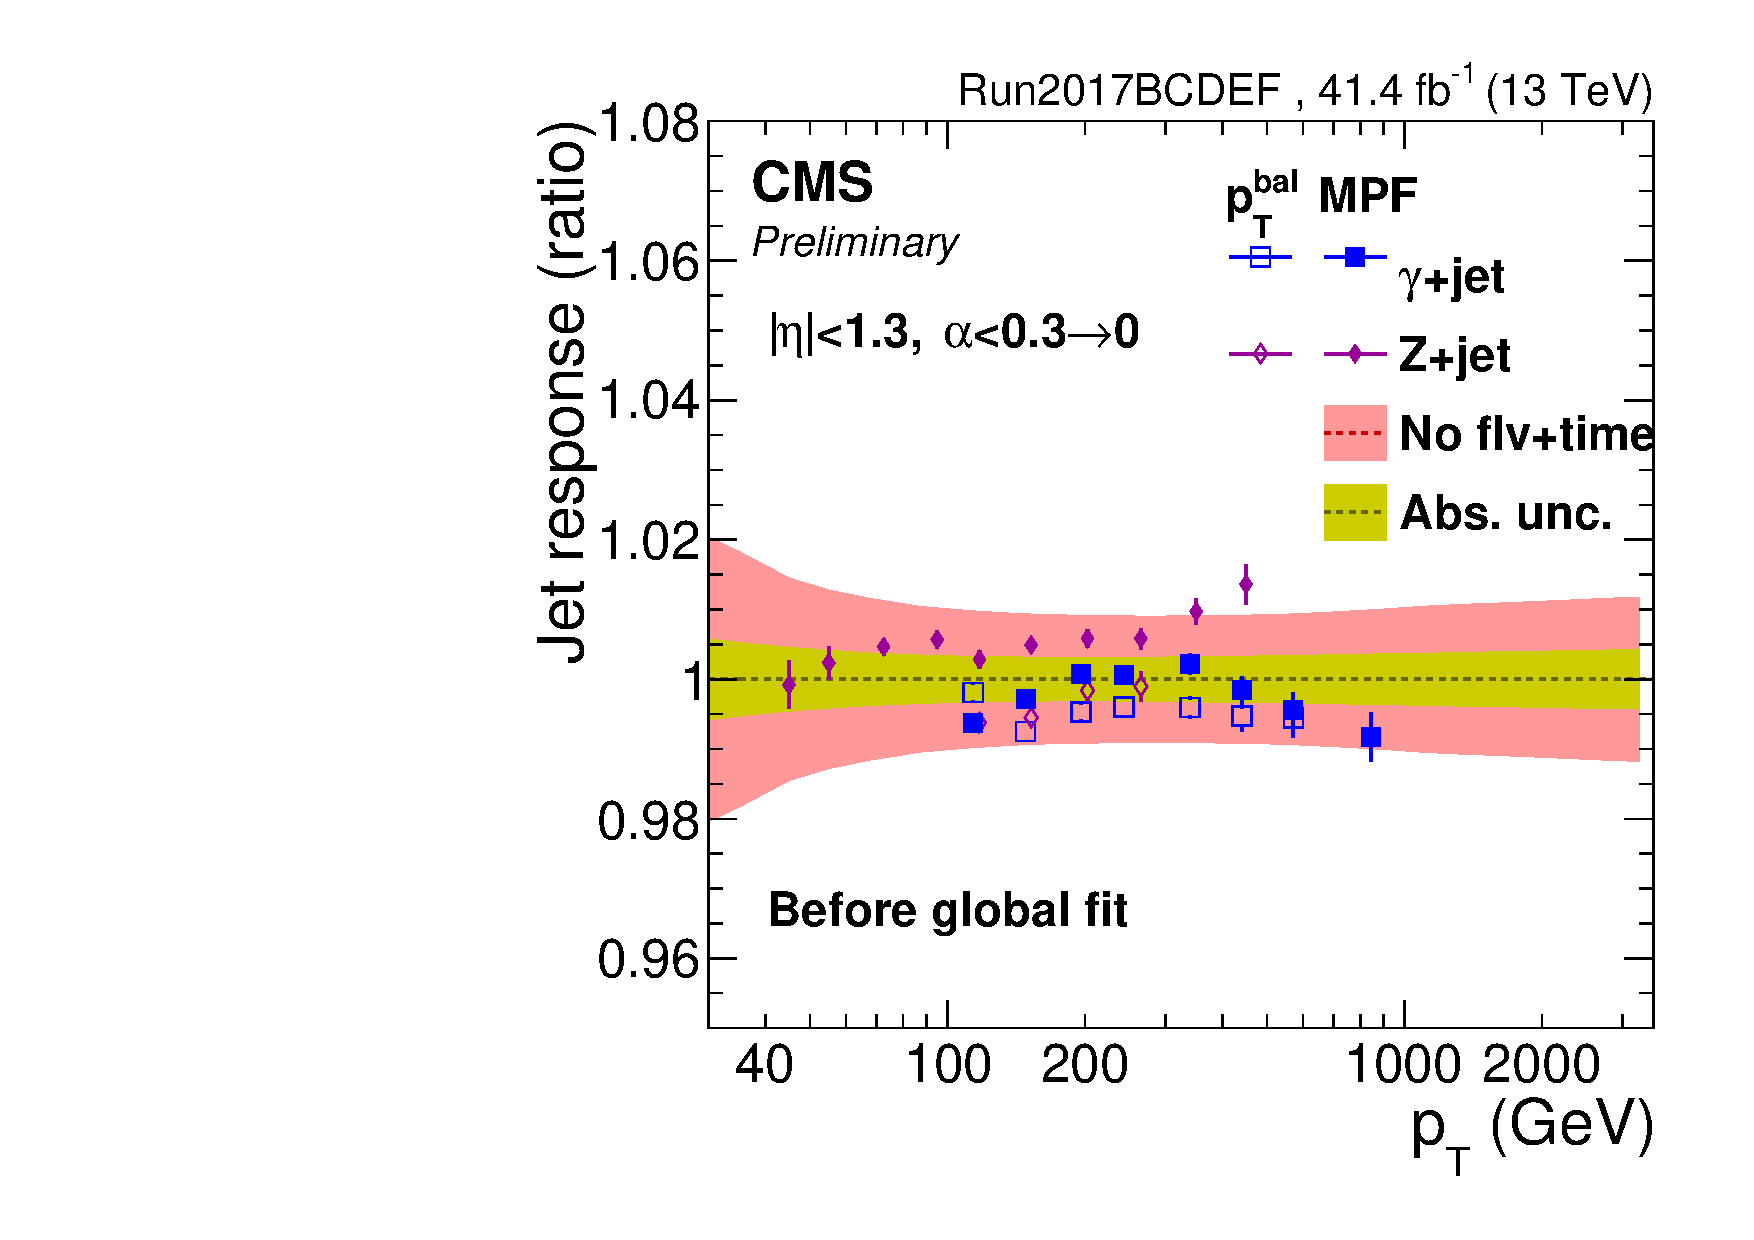
\includegraphics[width=0.32\textwidth]{BCDEFGH/globalFitL3res_orig.pdf}
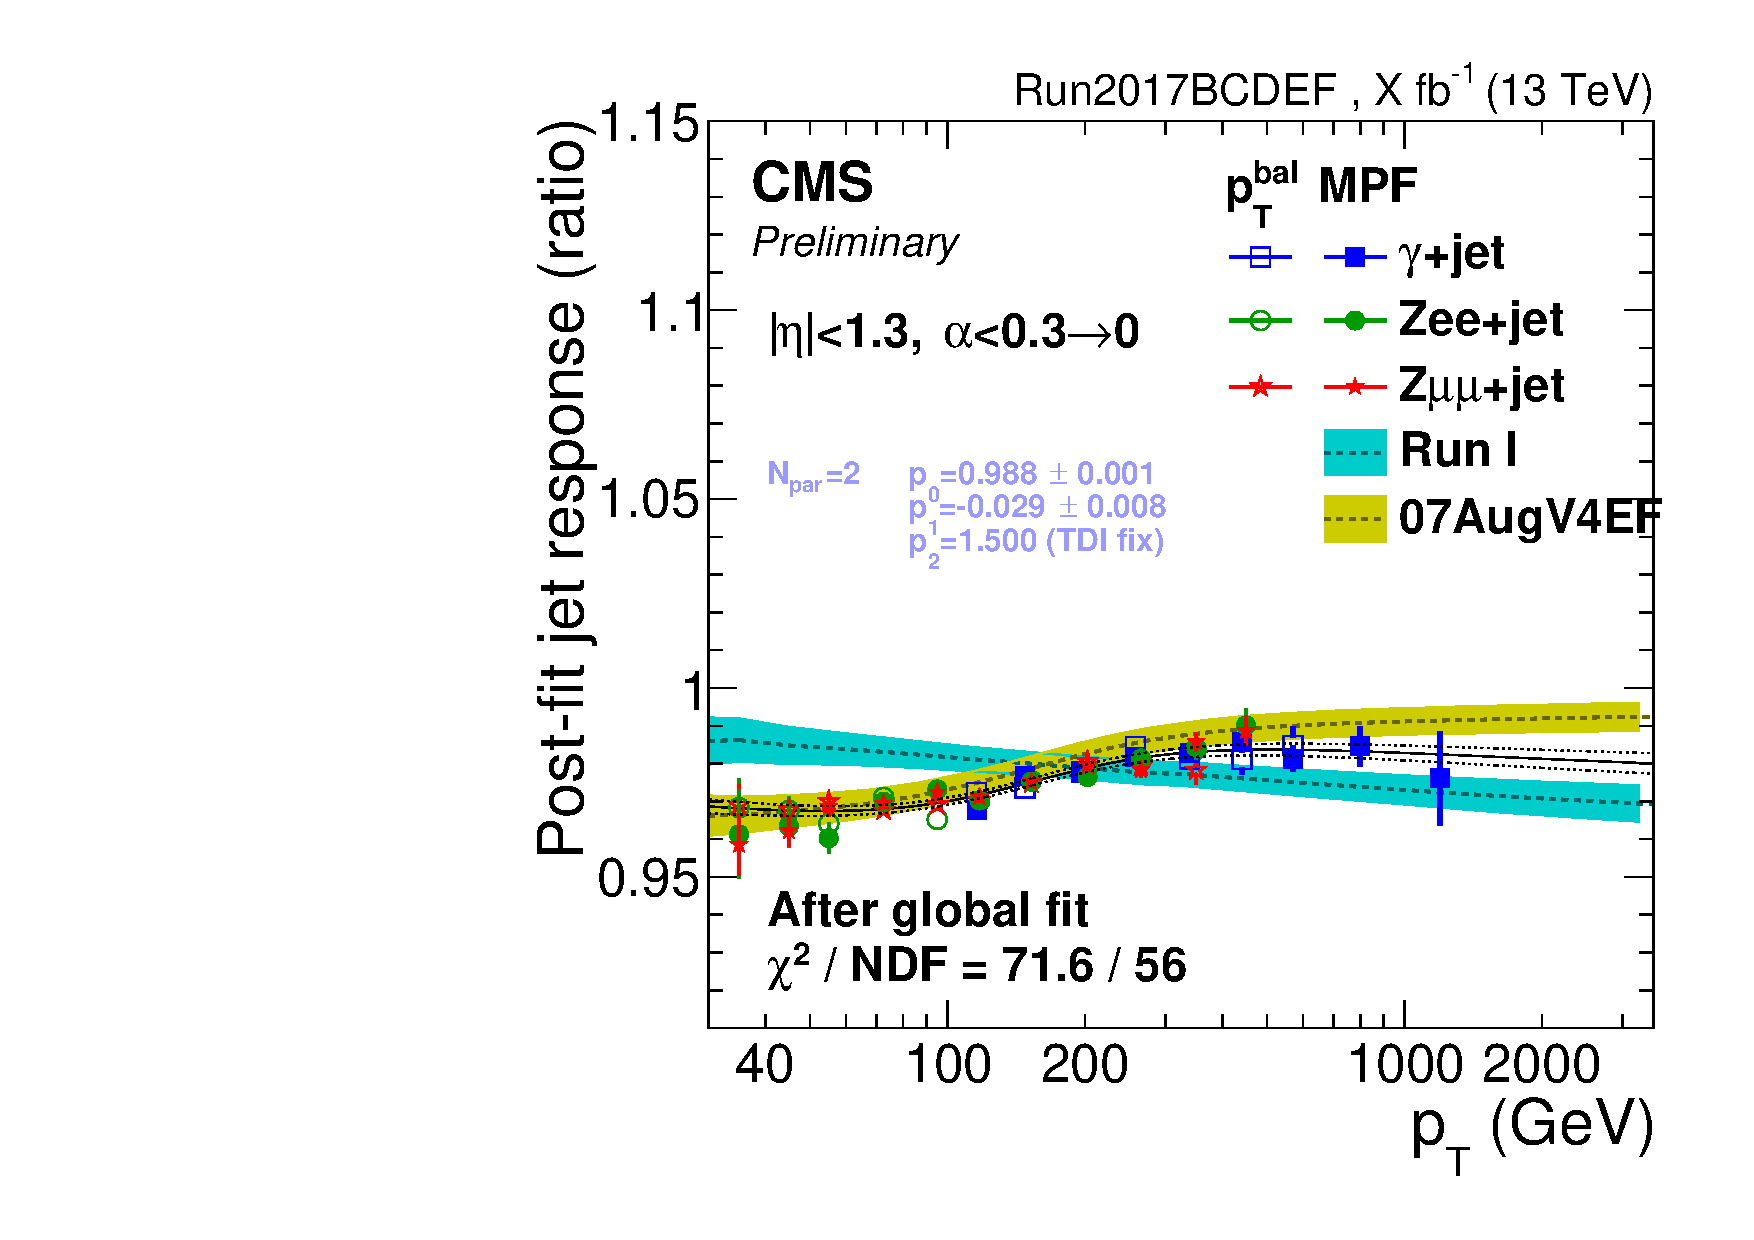
\includegraphics[width=0.32\textwidth]{BCDEFGH/globalFitL3res_shifted.pdf}\\
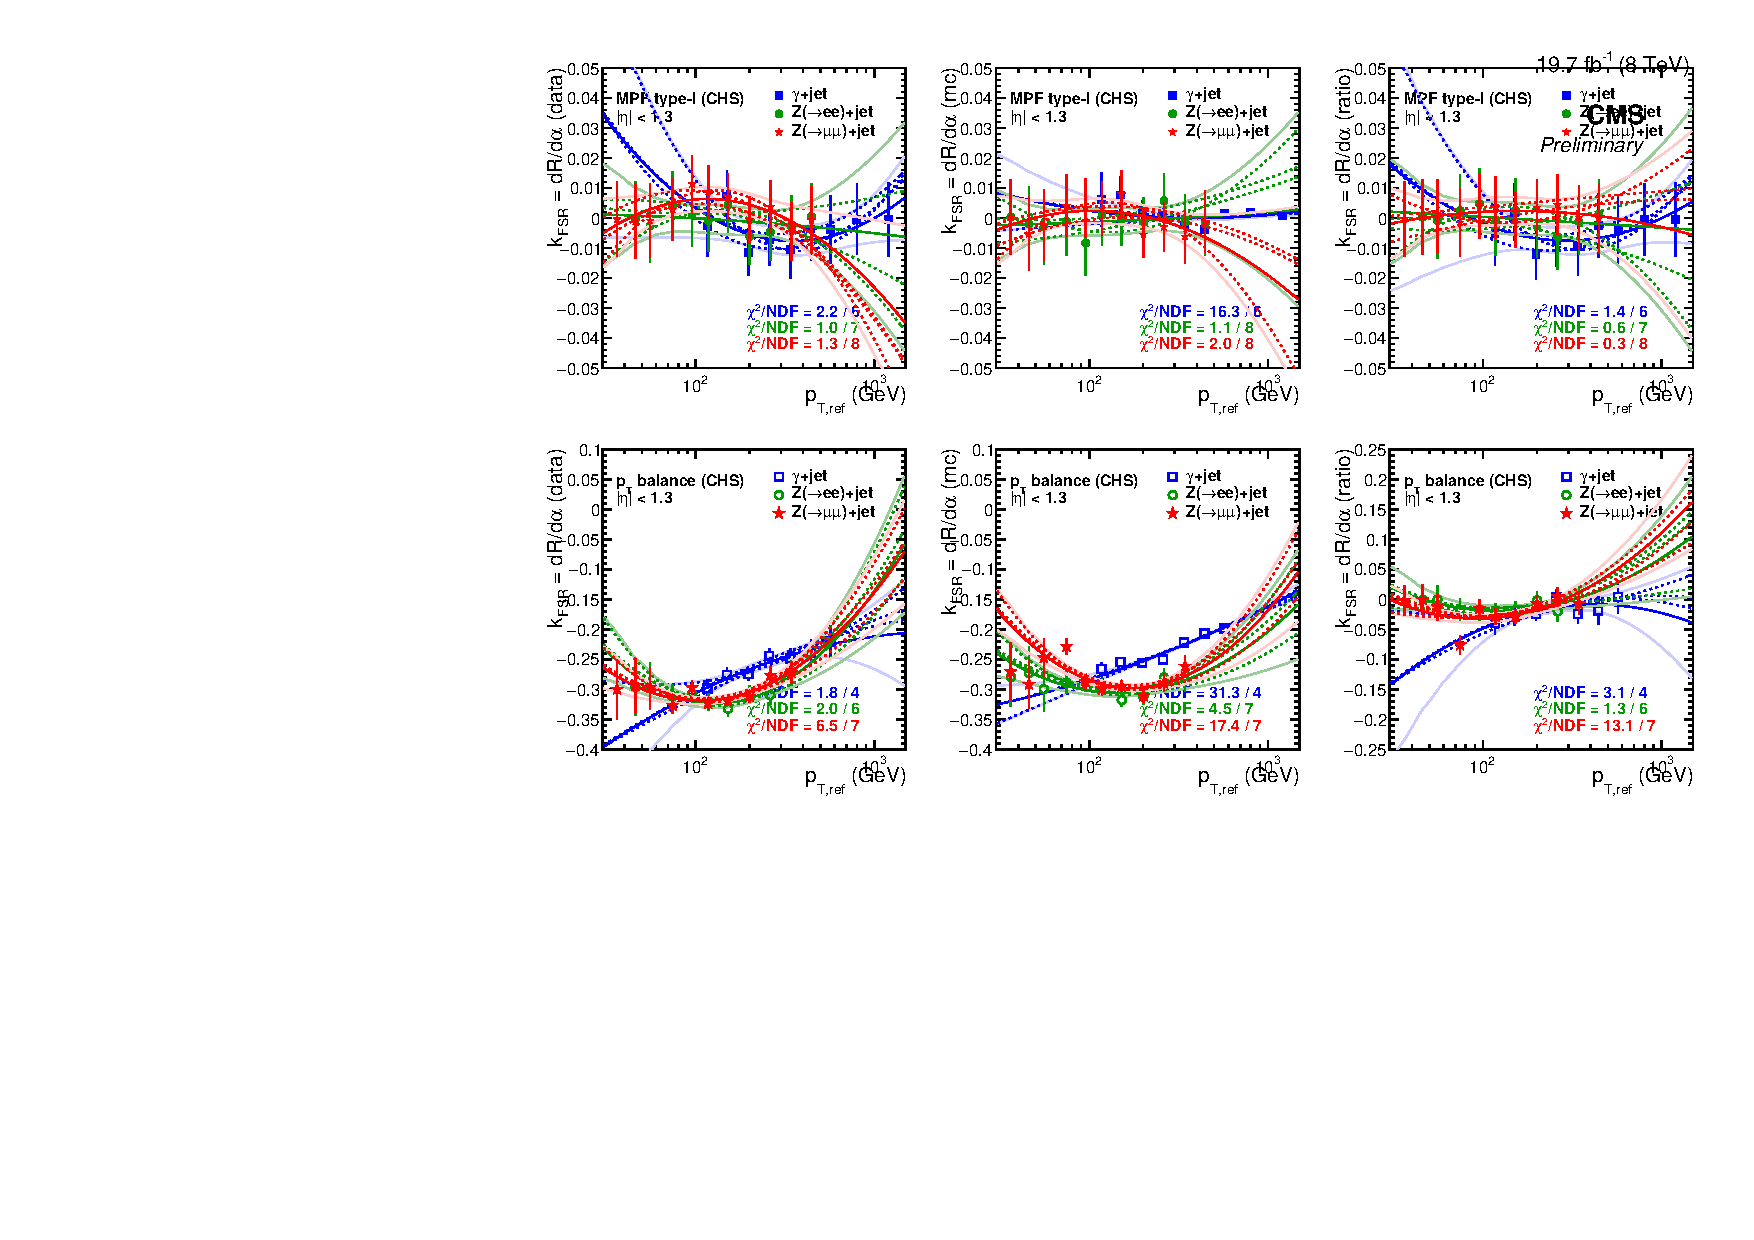
\includegraphics[width=0.30\textwidth]{BCDEFGH/softrad_2x6_kfsr_eta00-13.pdf}
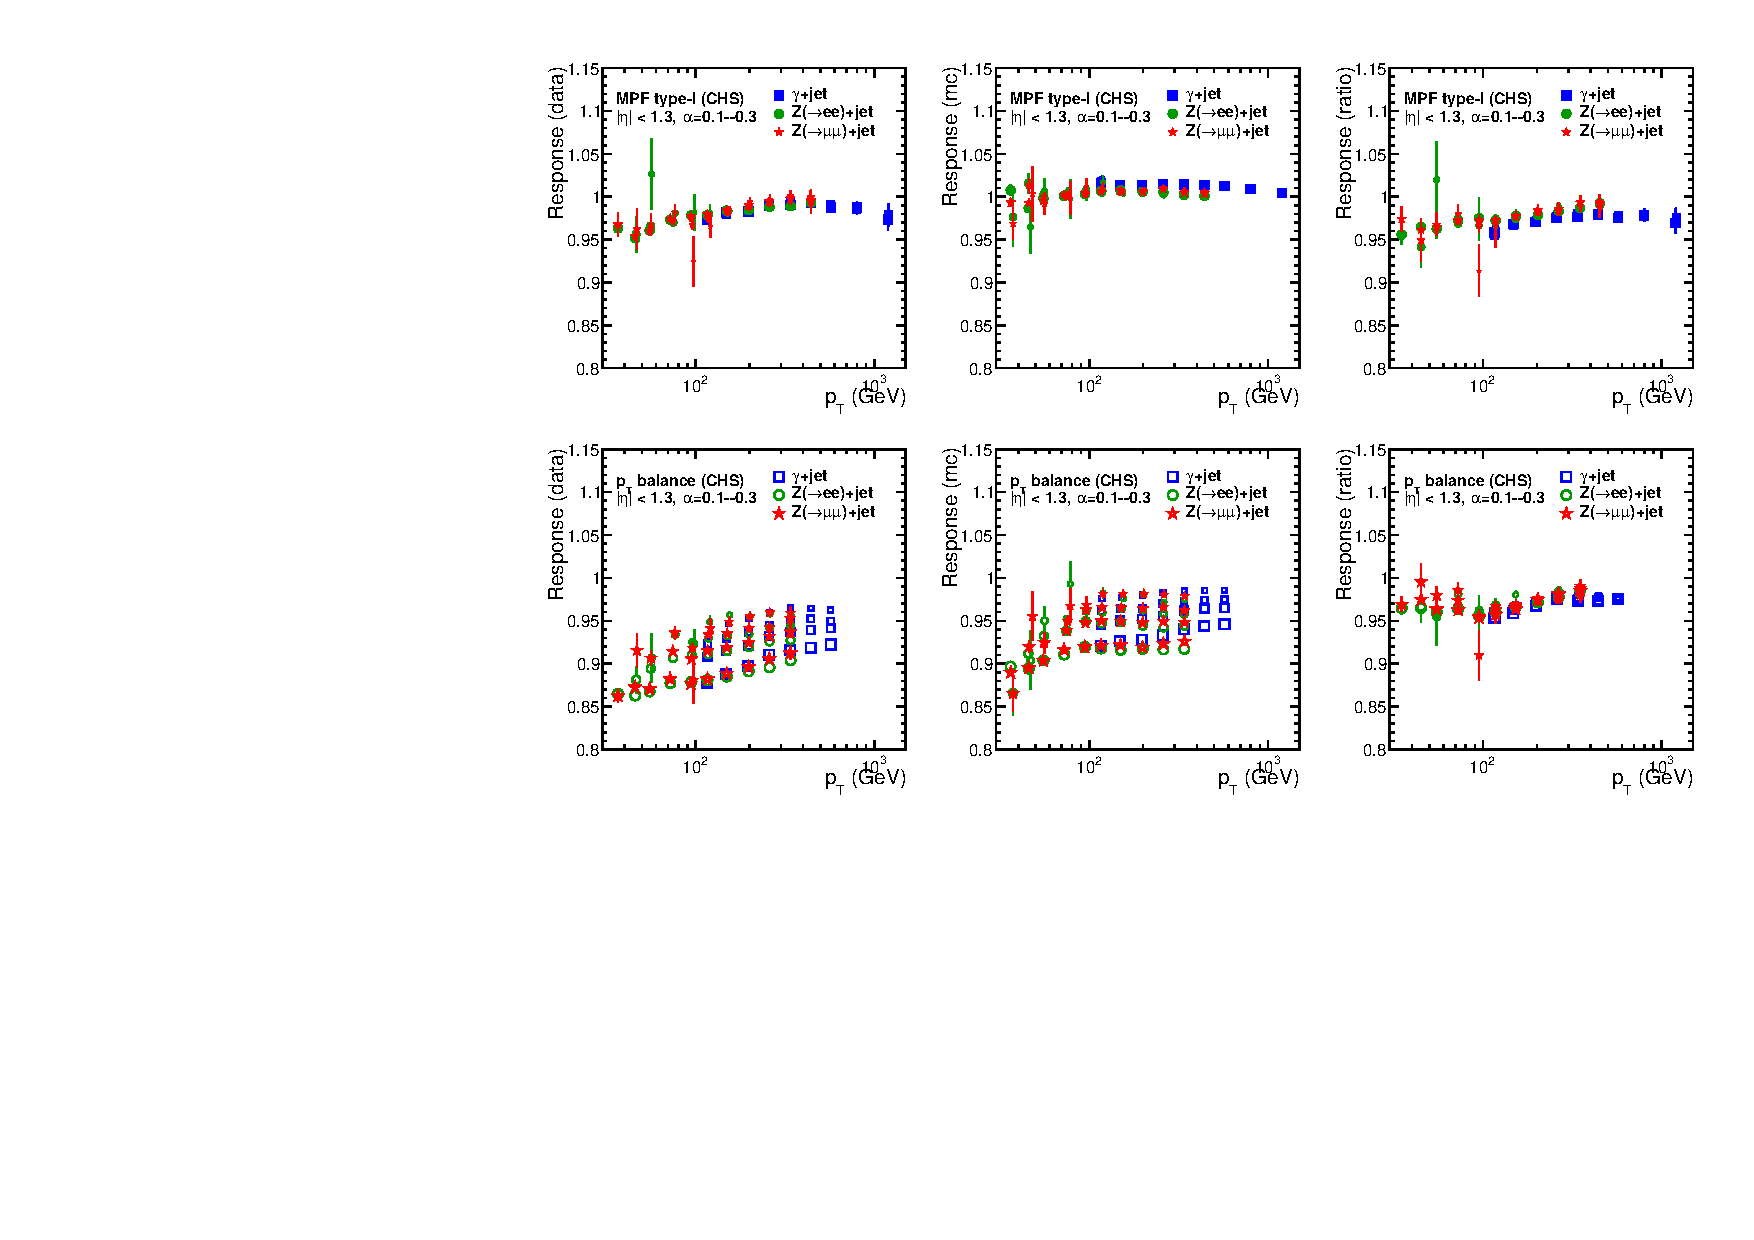
\includegraphics[width=0.30\textwidth]{BCDEFGH/softrad_2x6_vspt_eta00-13.pdf}
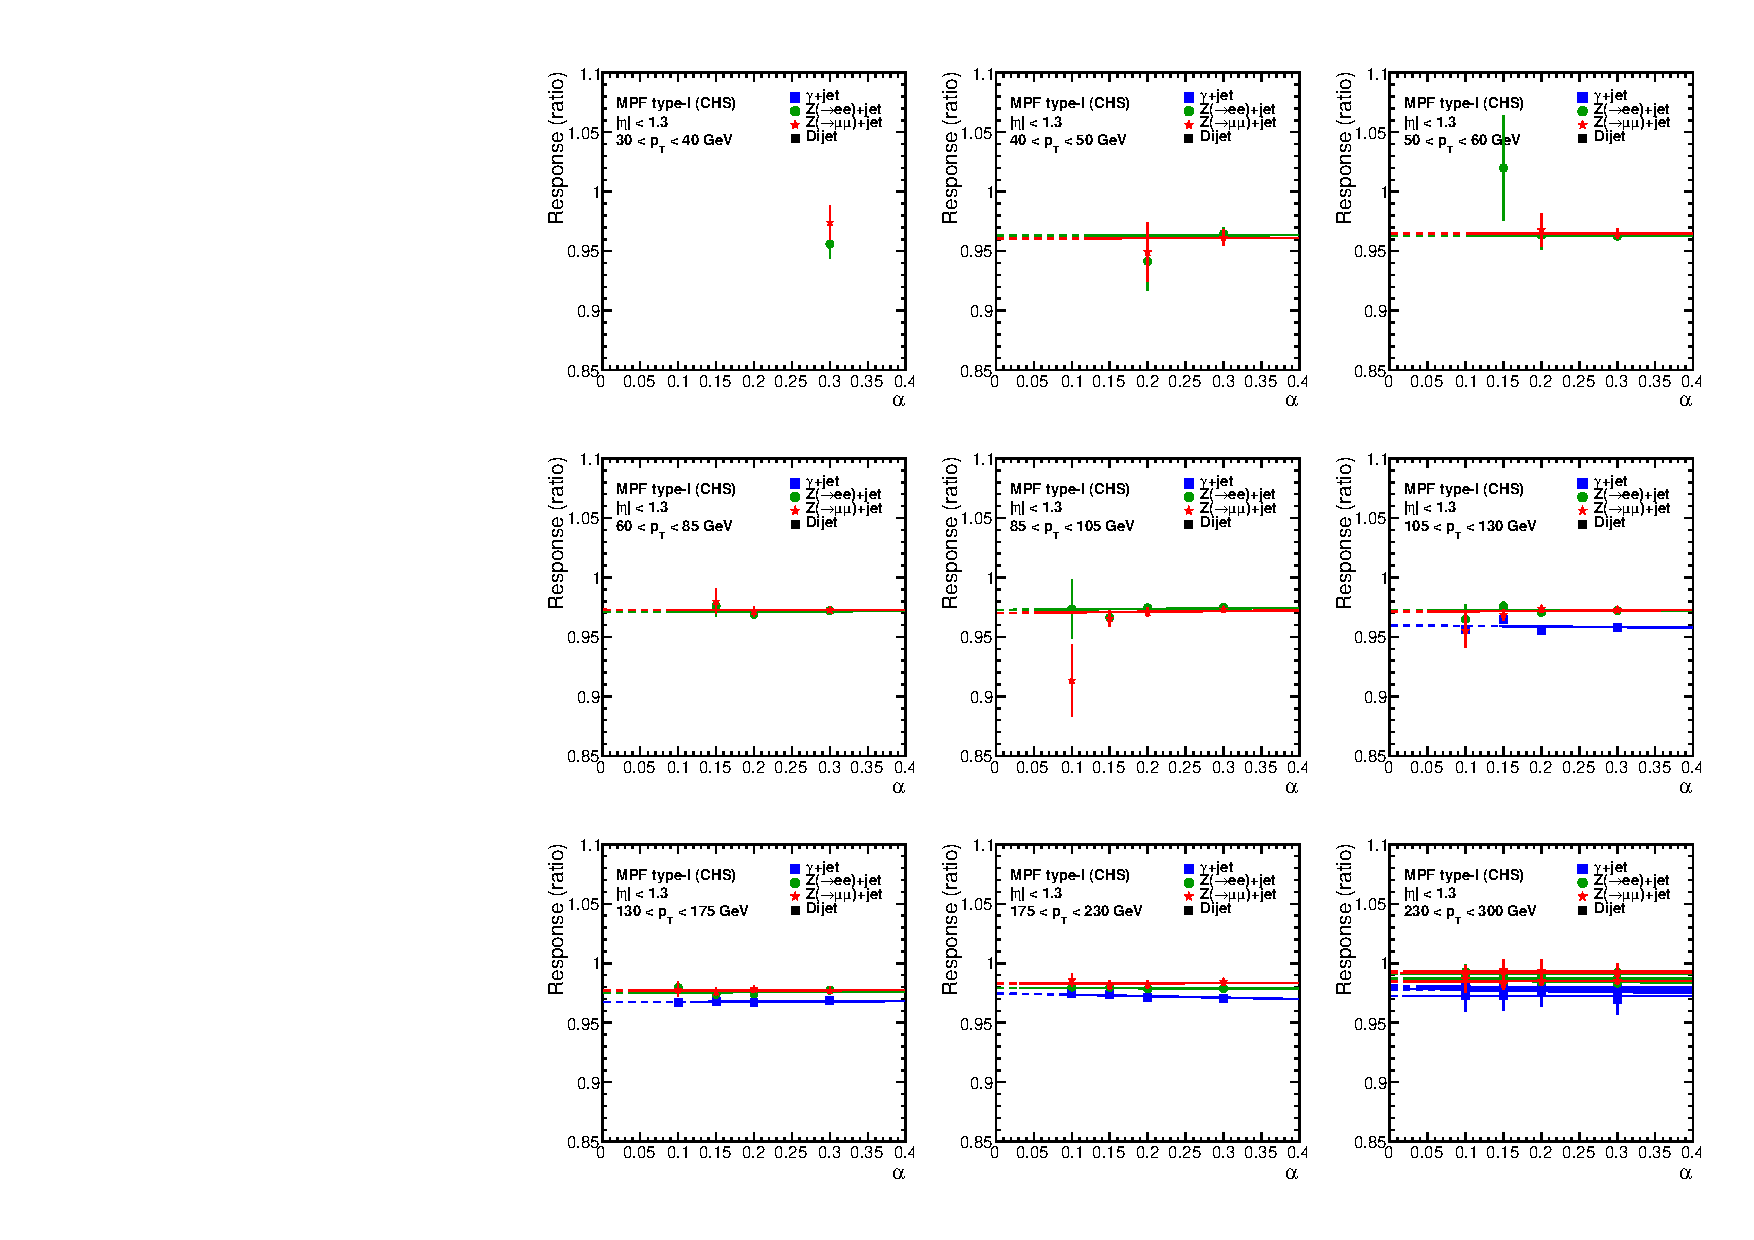
\includegraphics[width=0.20\textwidth]{BCDEFGH/softrad_3x3_ratio_mpfchs1_vsalpha_eta00-13.pdf}
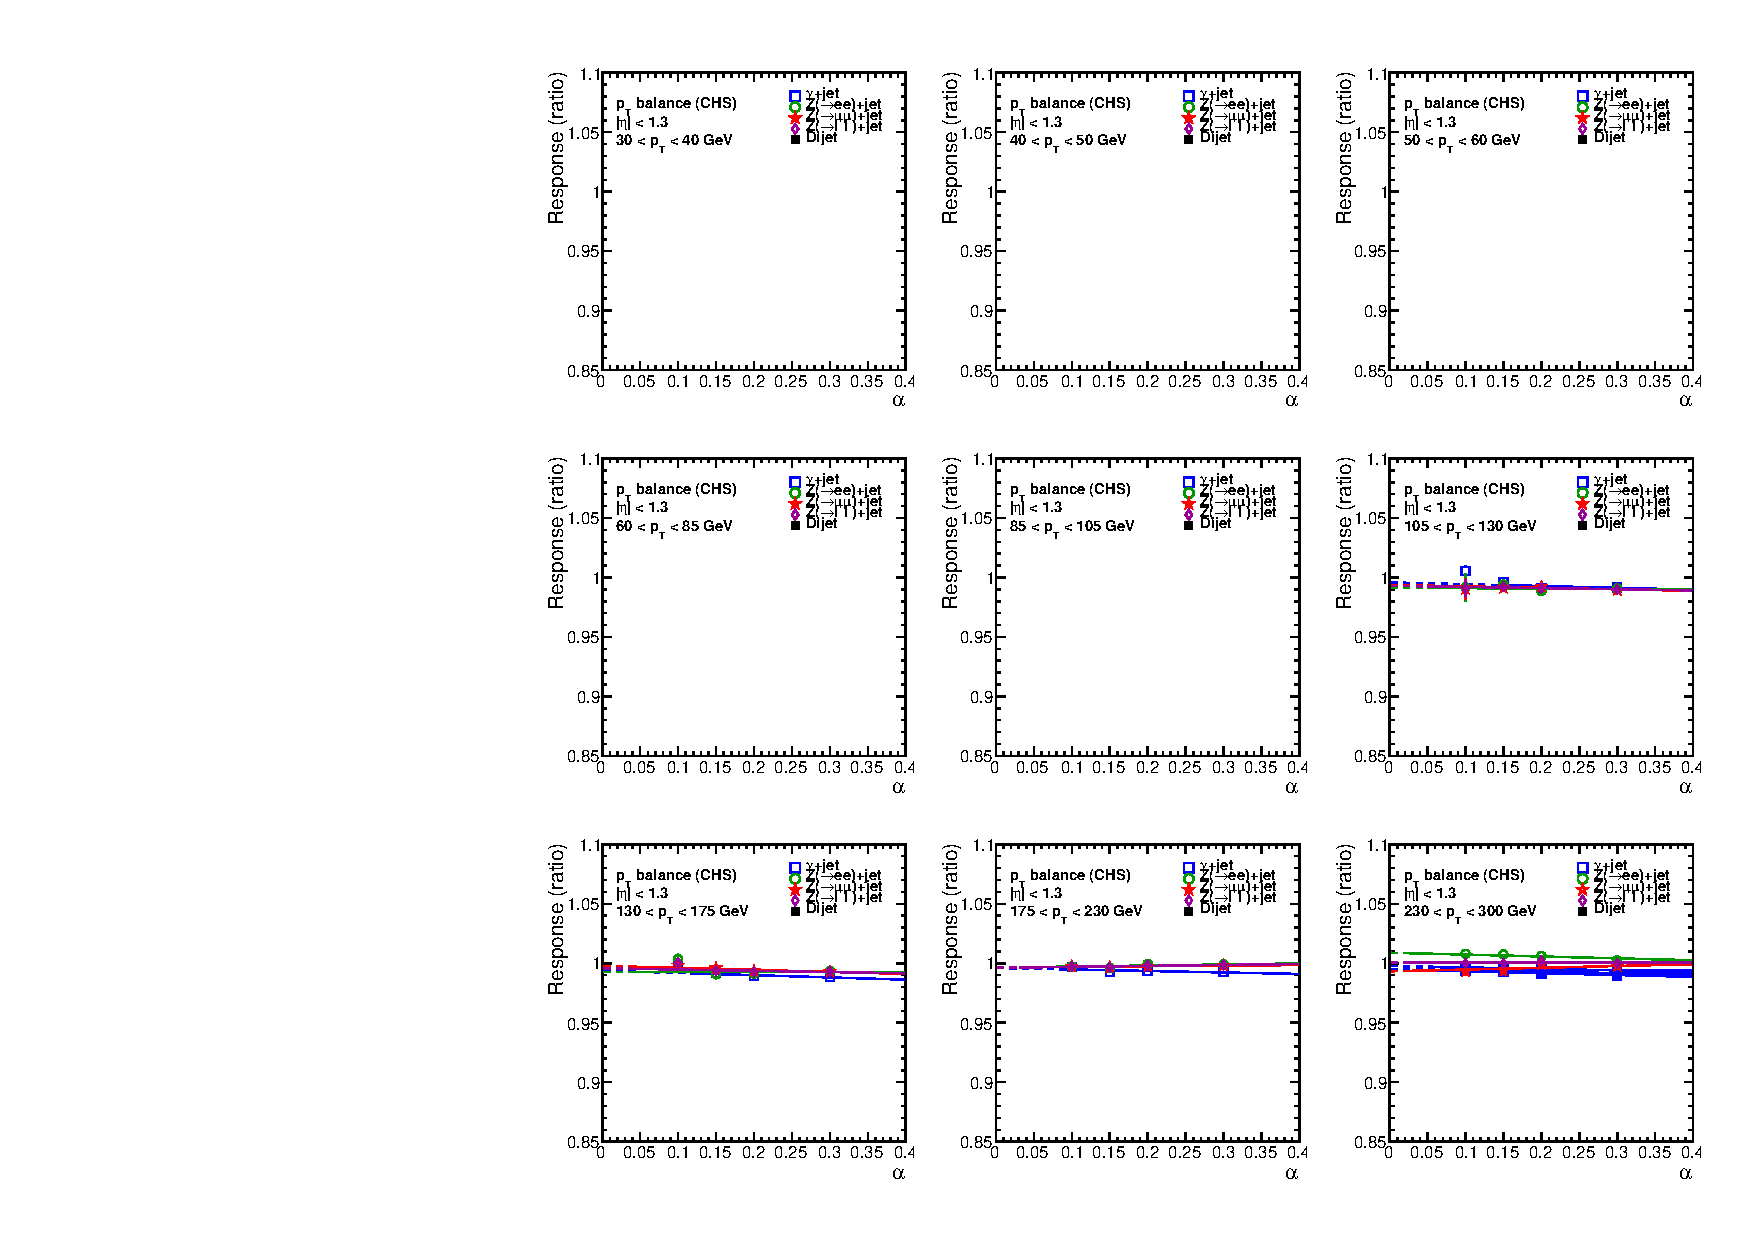
\includegraphics[width=0.20\textwidth]{BCDEFGH/softrad_3x3_ratio_ptchs_vsalpha_eta00-13.pdf}\\

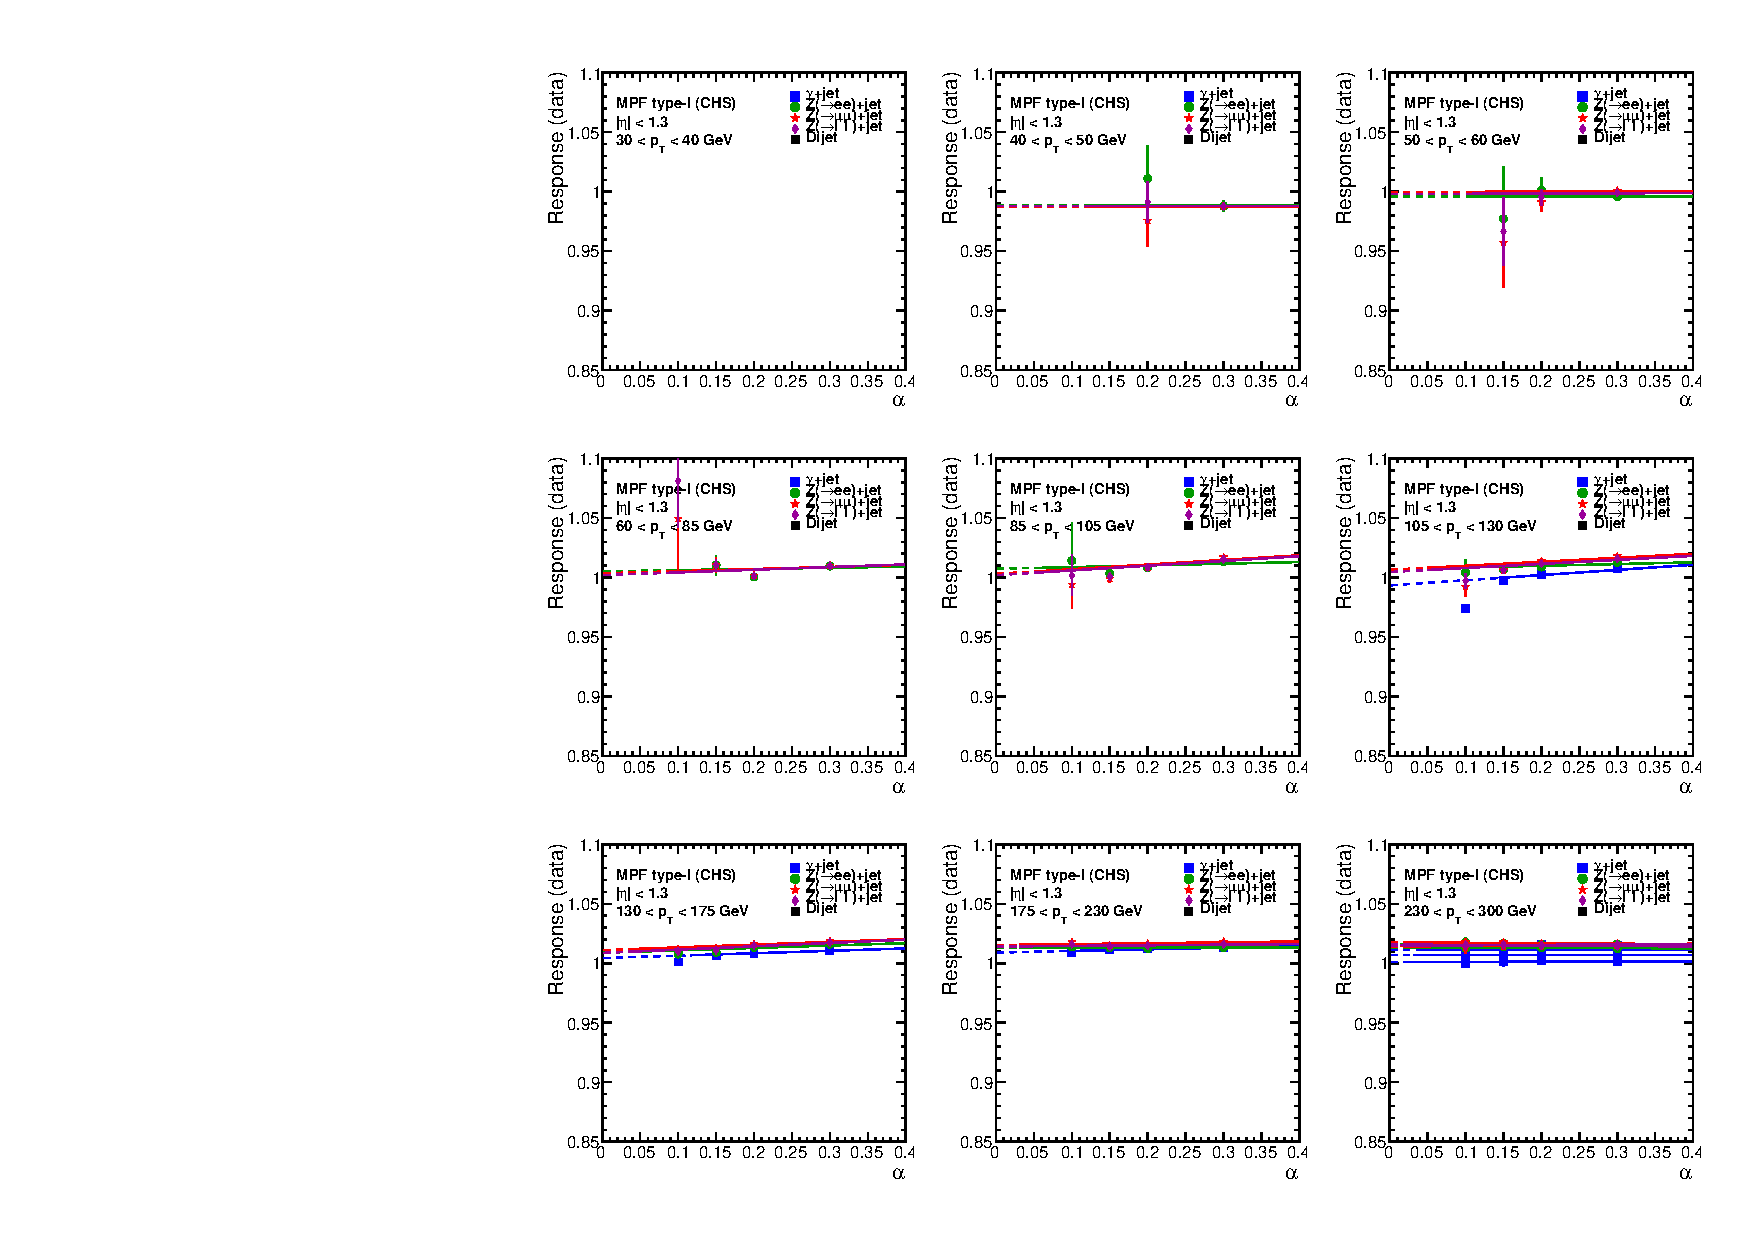
\includegraphics[width=0.15\textwidth]{BCDEFGH/softrad_3x3_data_mpfchs1_vsalpha_eta00-13.pdf}
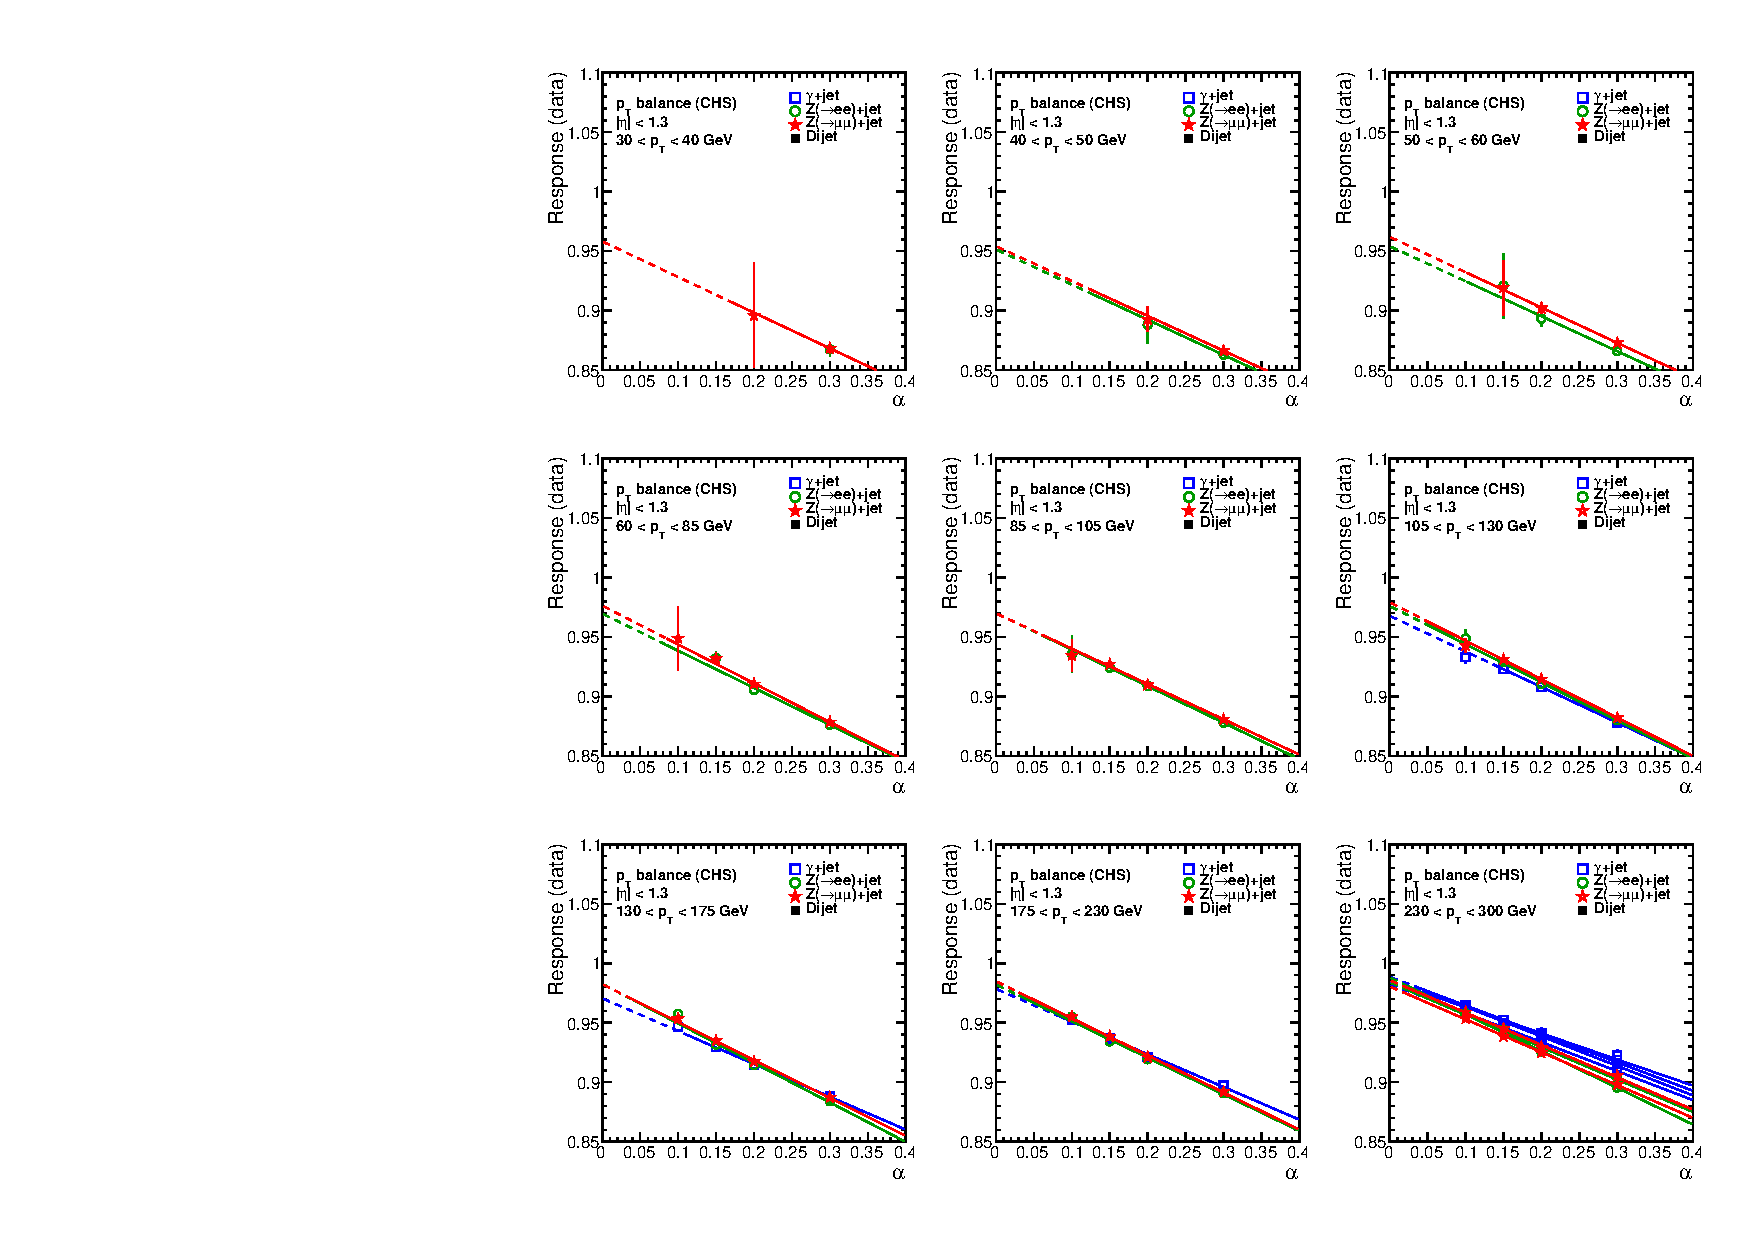
\includegraphics[width=0.15\textwidth]{BCDEFGH/softrad_3x3_data_ptchs_vsalpha_eta00-13.pdf}
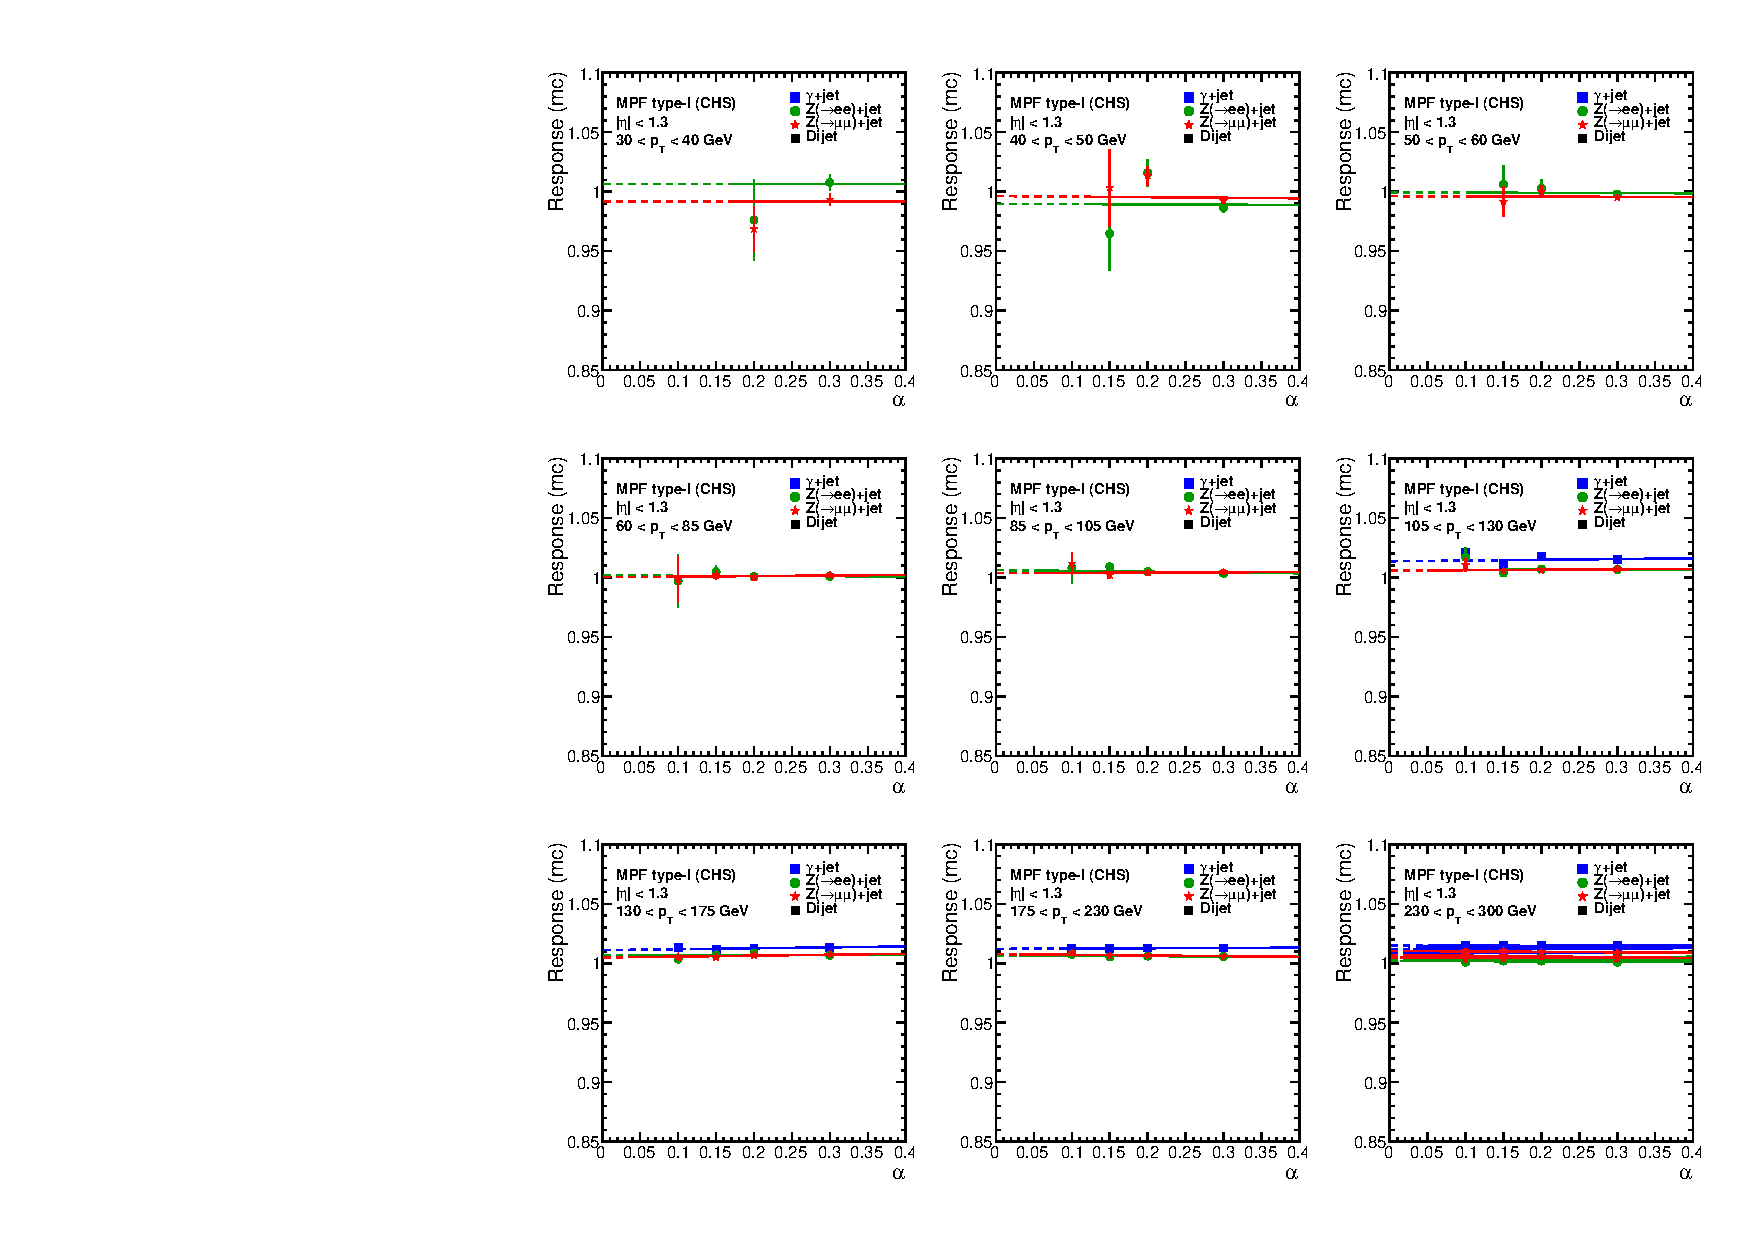
\includegraphics[width=0.15\textwidth]{BCDEFGH/softrad_3x3_mc_mpfchs1_vsalpha_eta00-13.pdf} 
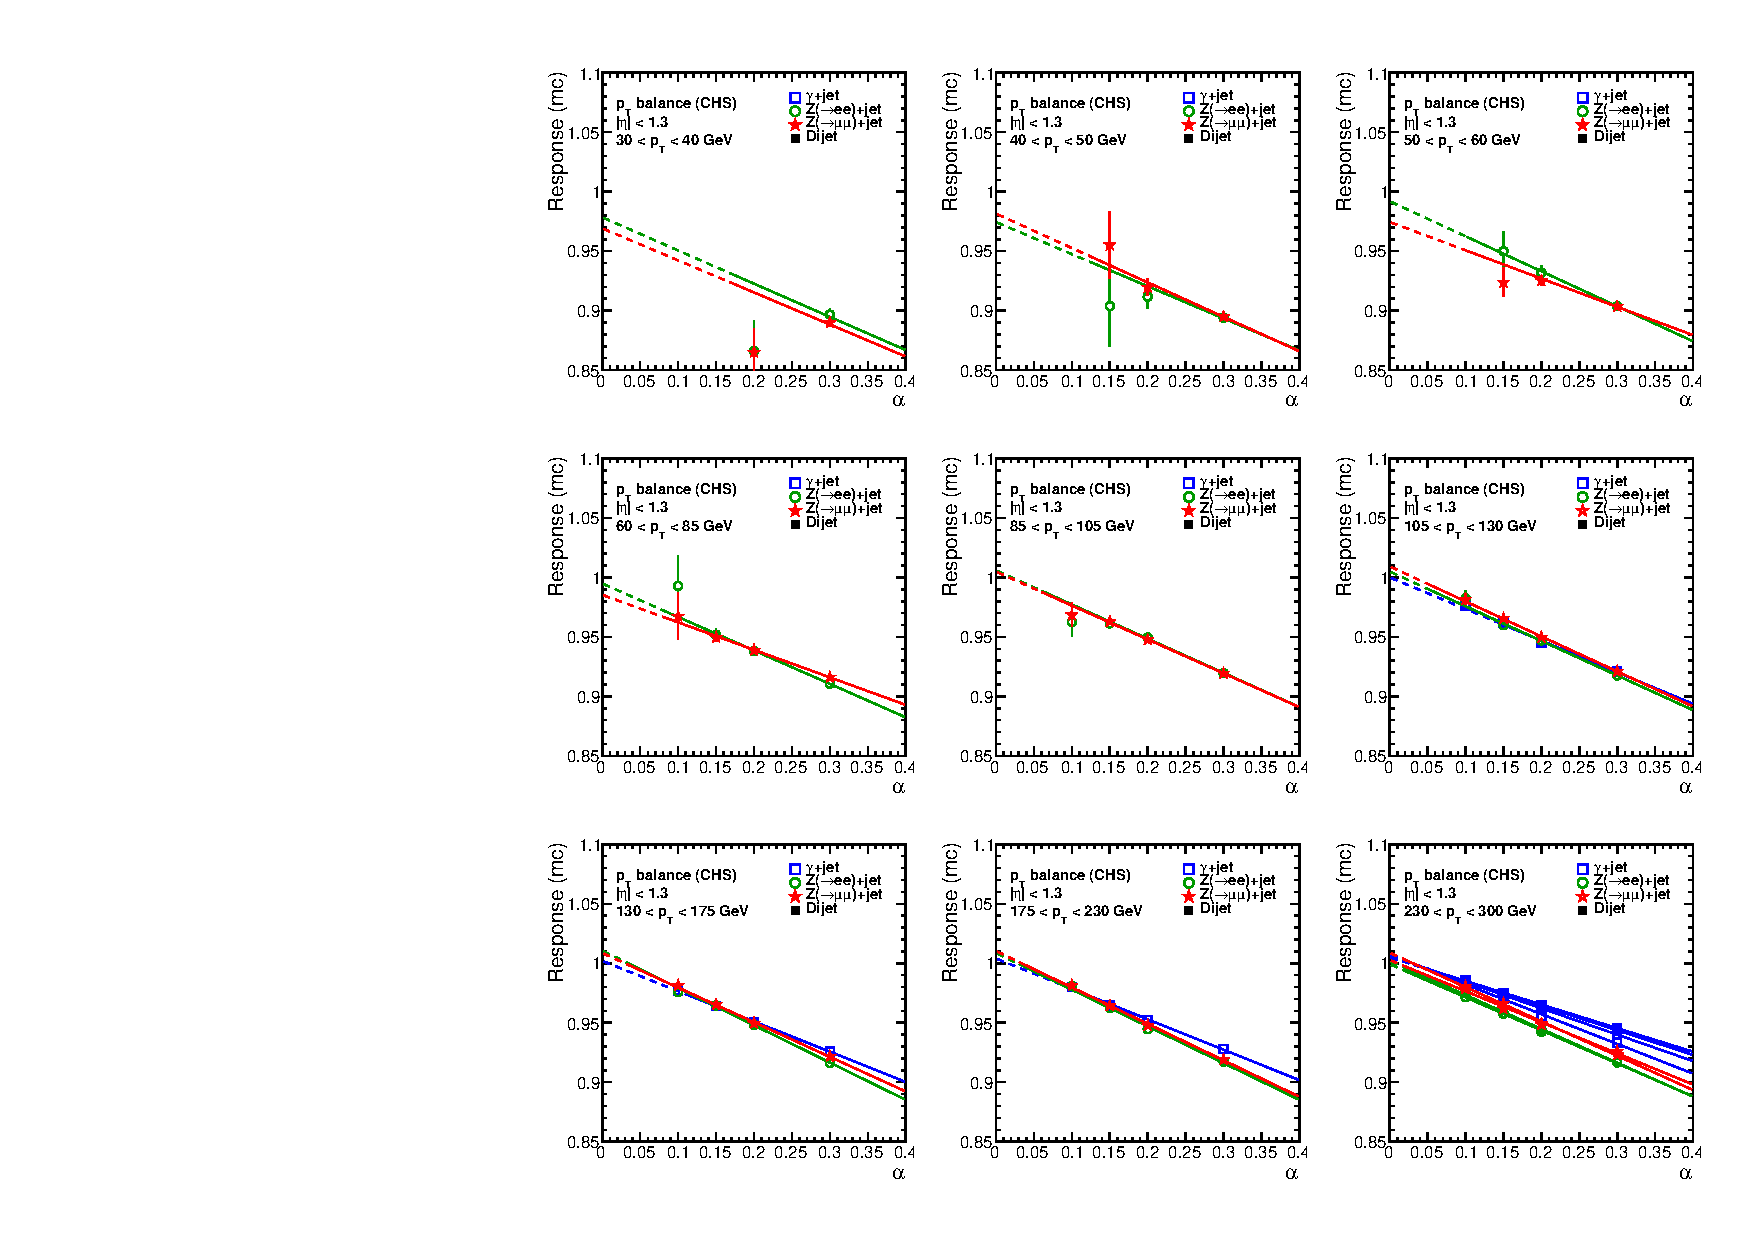
\includegraphics[width=0.15\textwidth]{BCDEFGH/softrad_3x3_mc_ptchs_vsalpha_eta00-13.pdf}  
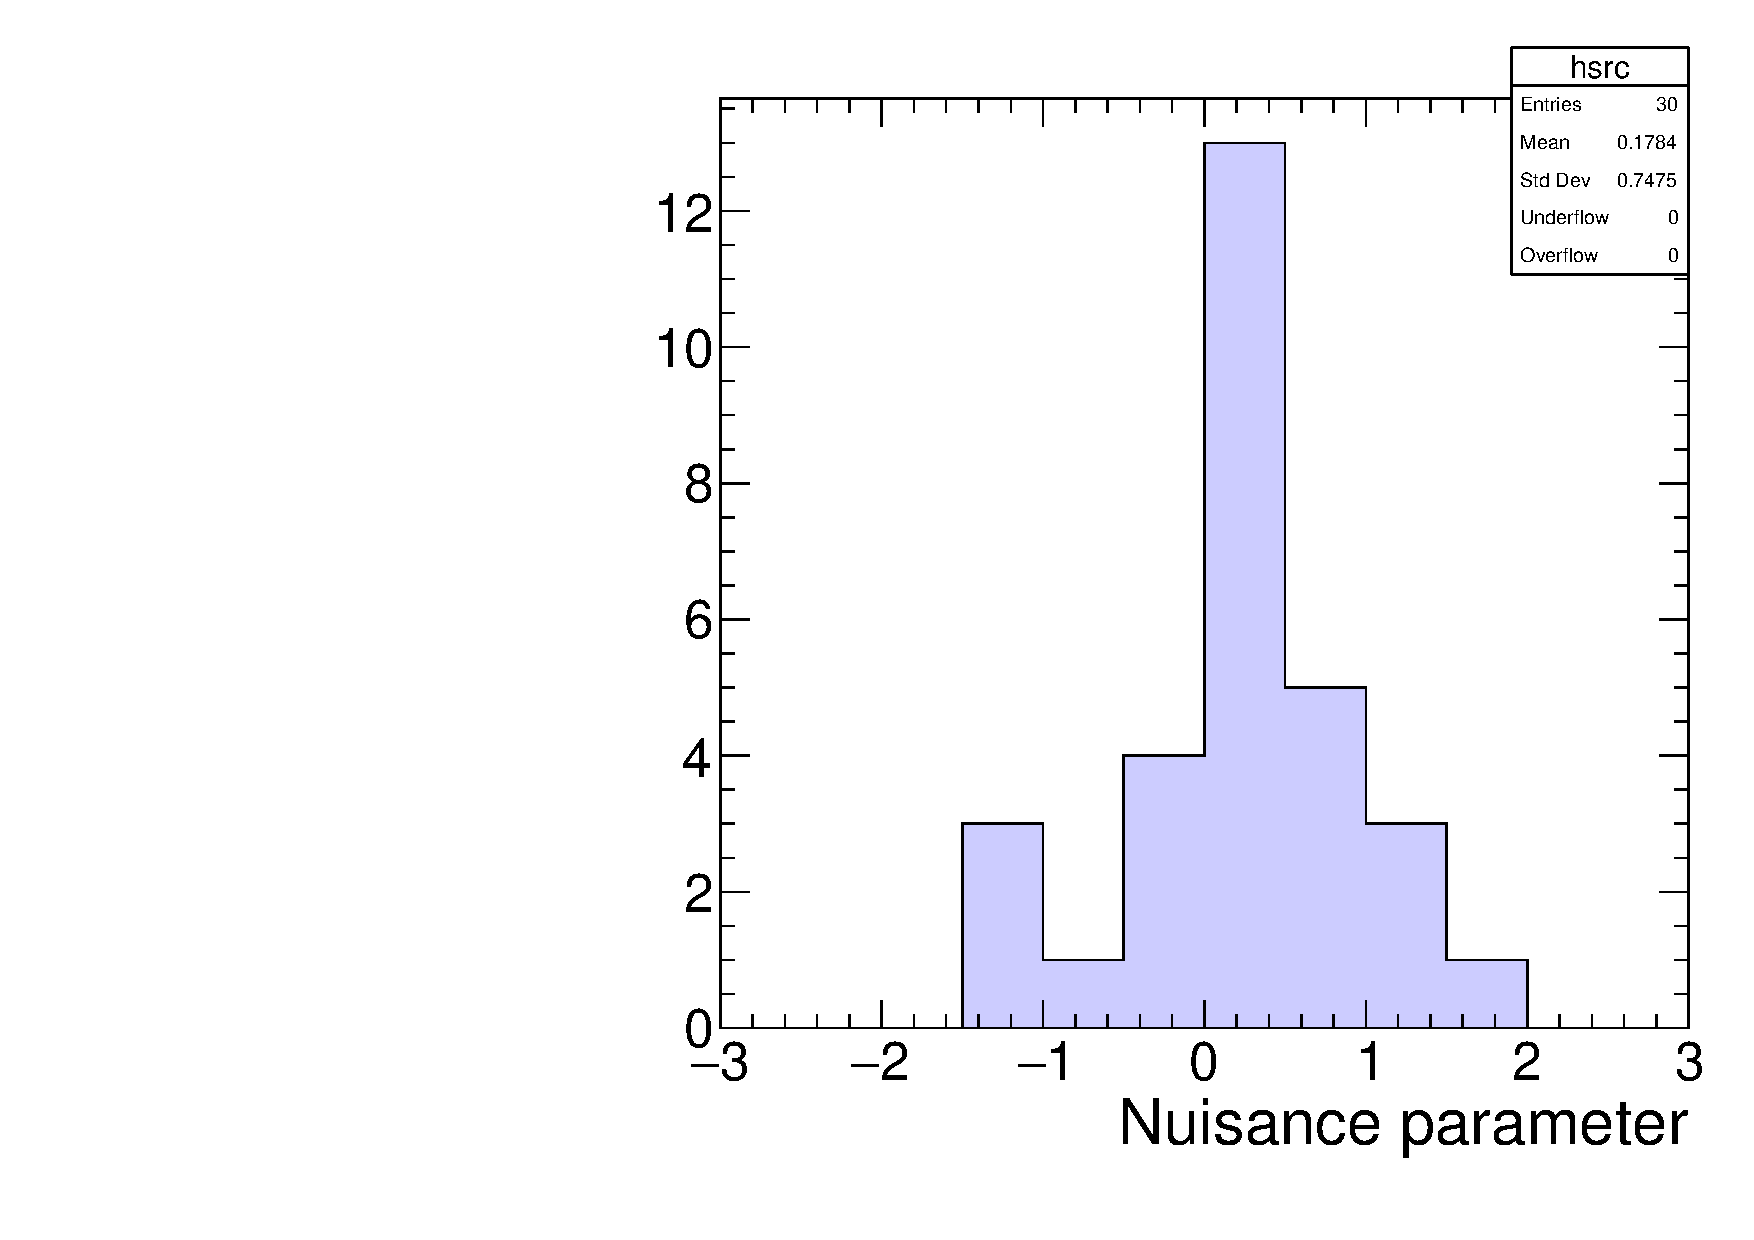
\includegraphics[width=0.10\textwidth]{BCDEFGH/globalFitL3res_hsrc.pdf}
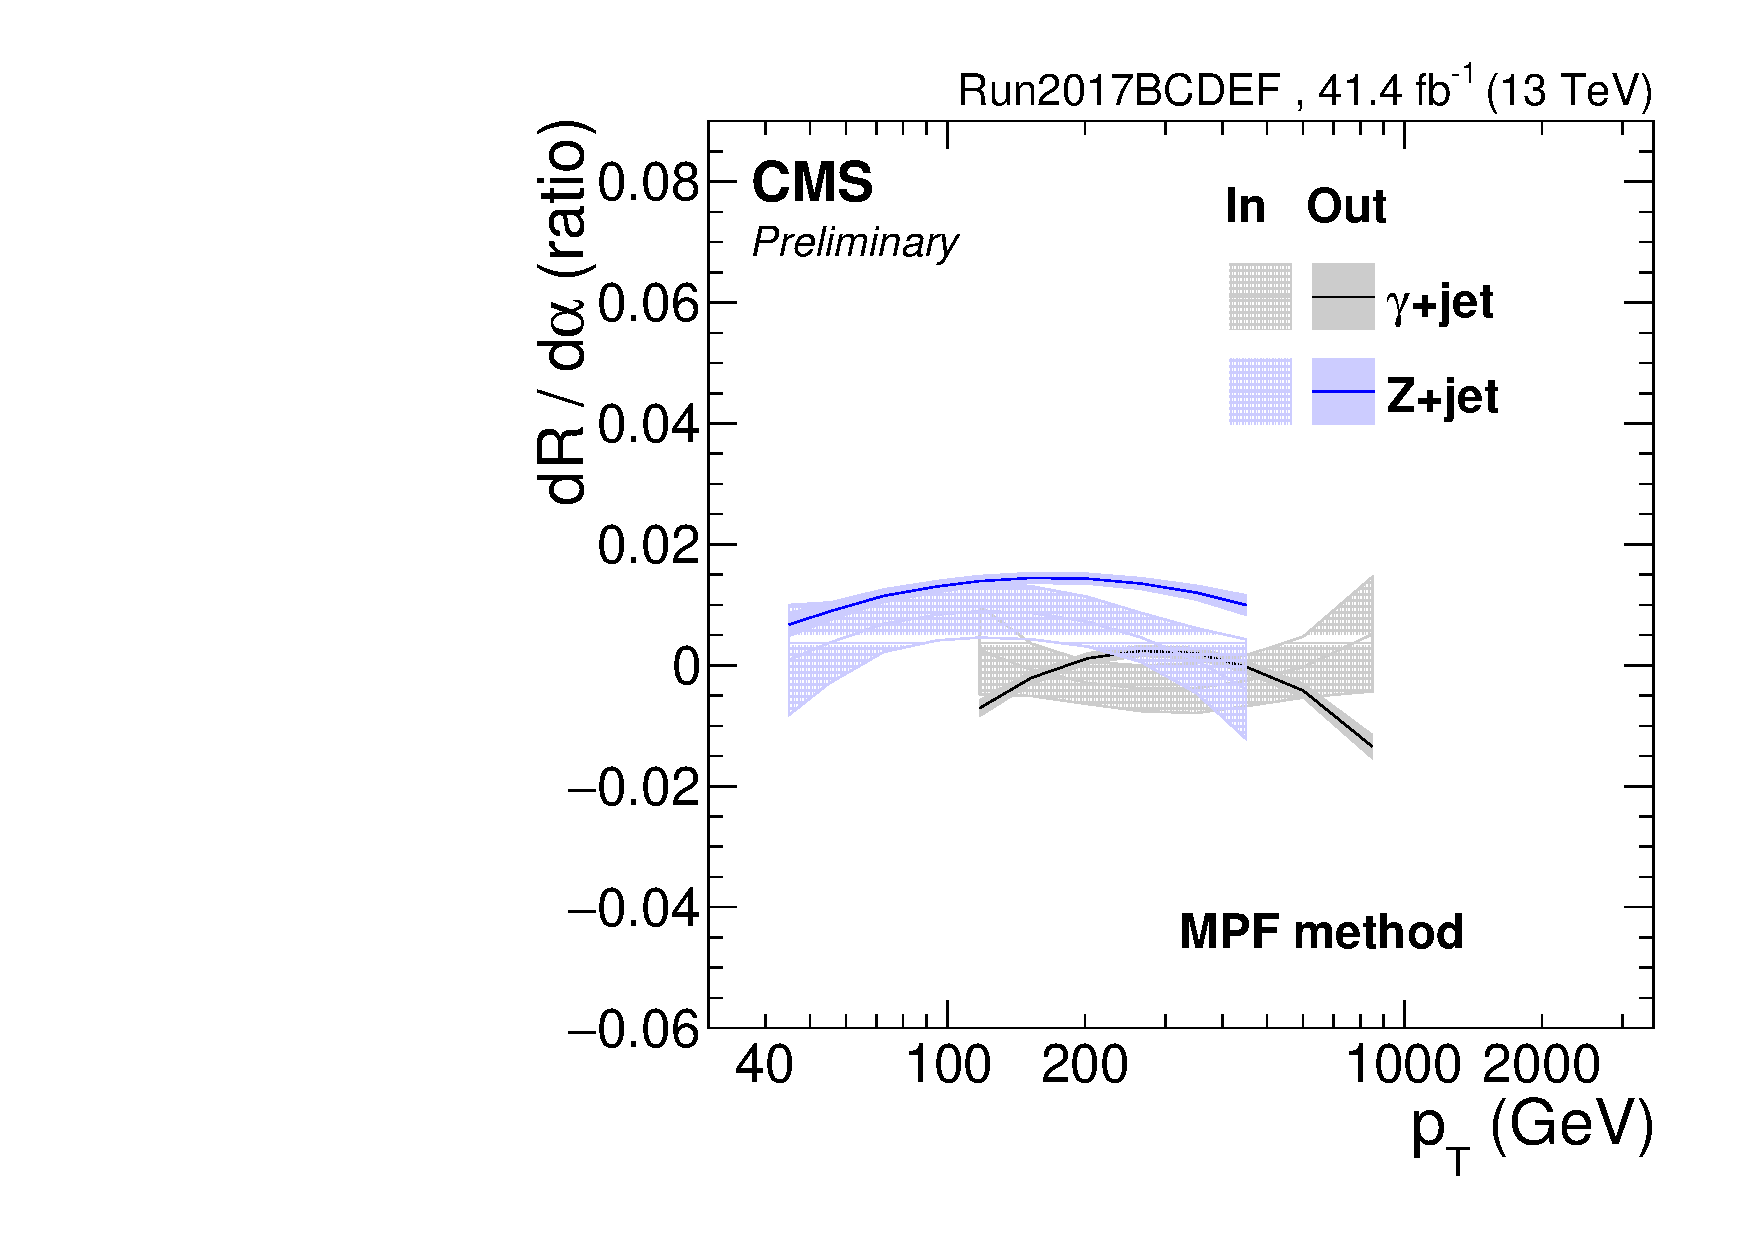
\includegraphics[width=0.10\textwidth]{BCDEFGH/globalFitL3res_mpfchs1_kfsr.pdf}
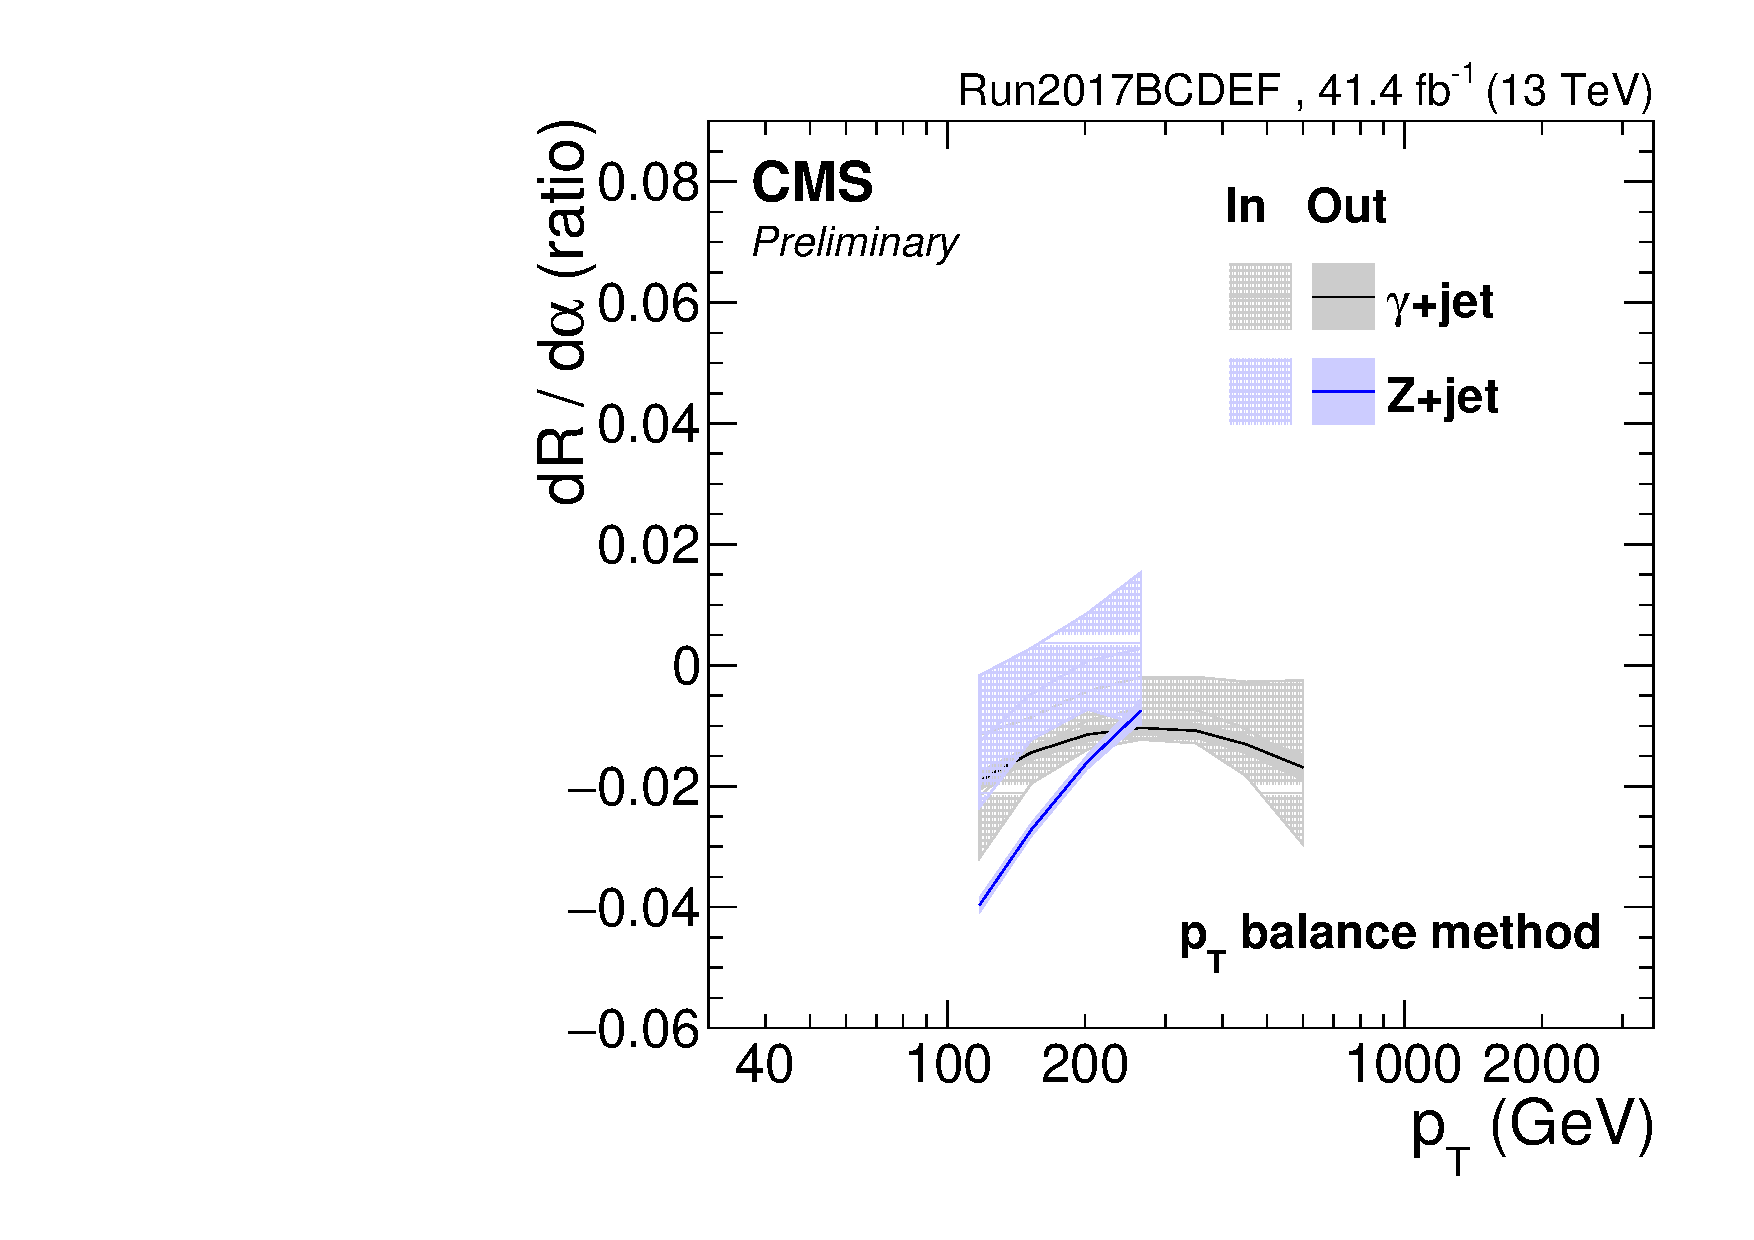
\includegraphics[width=0.10\textwidth]{BCDEFGH/globalFitL3res_ptchs_kfsr.pdf}\\

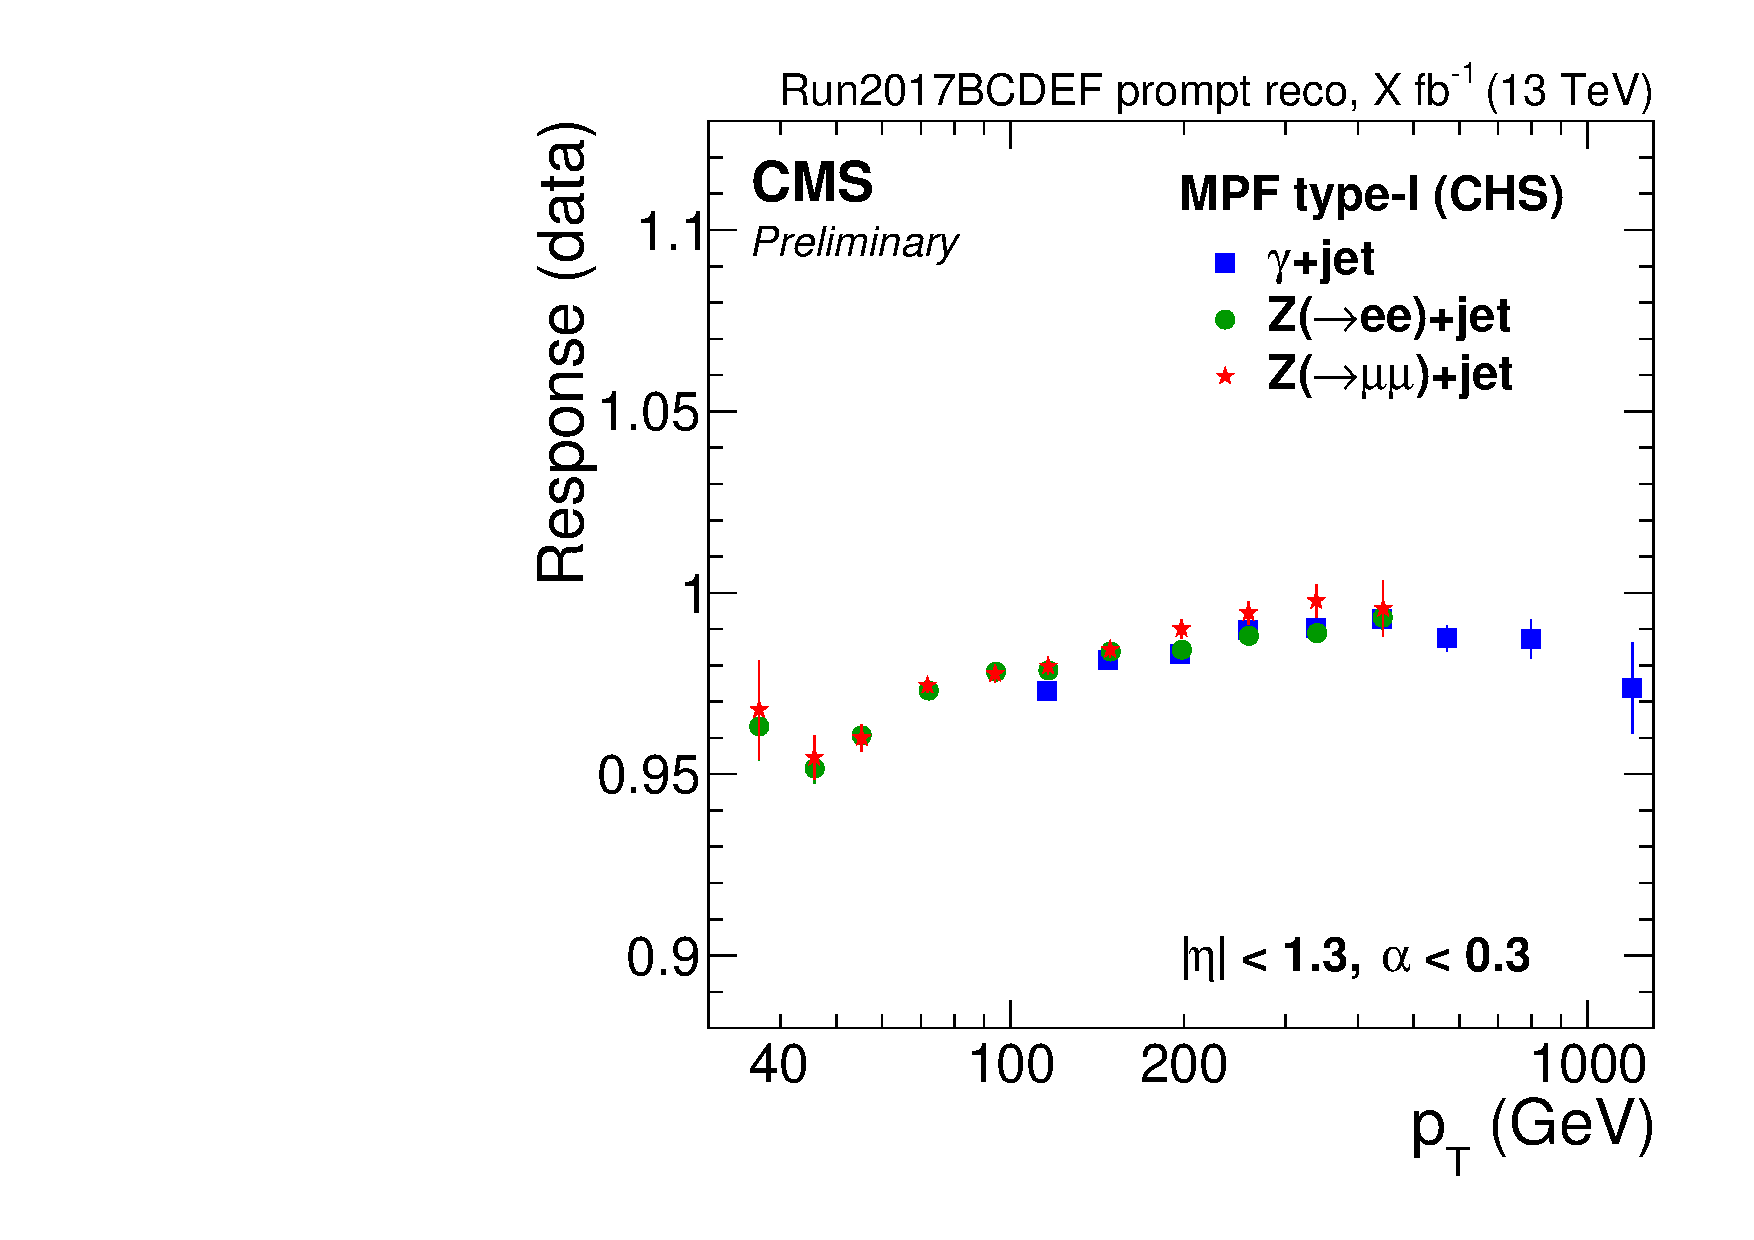
\includegraphics[width=0.10\textwidth]{BCDEFGH/paper_softrad_data_mpfchs1_vspt.pdf}
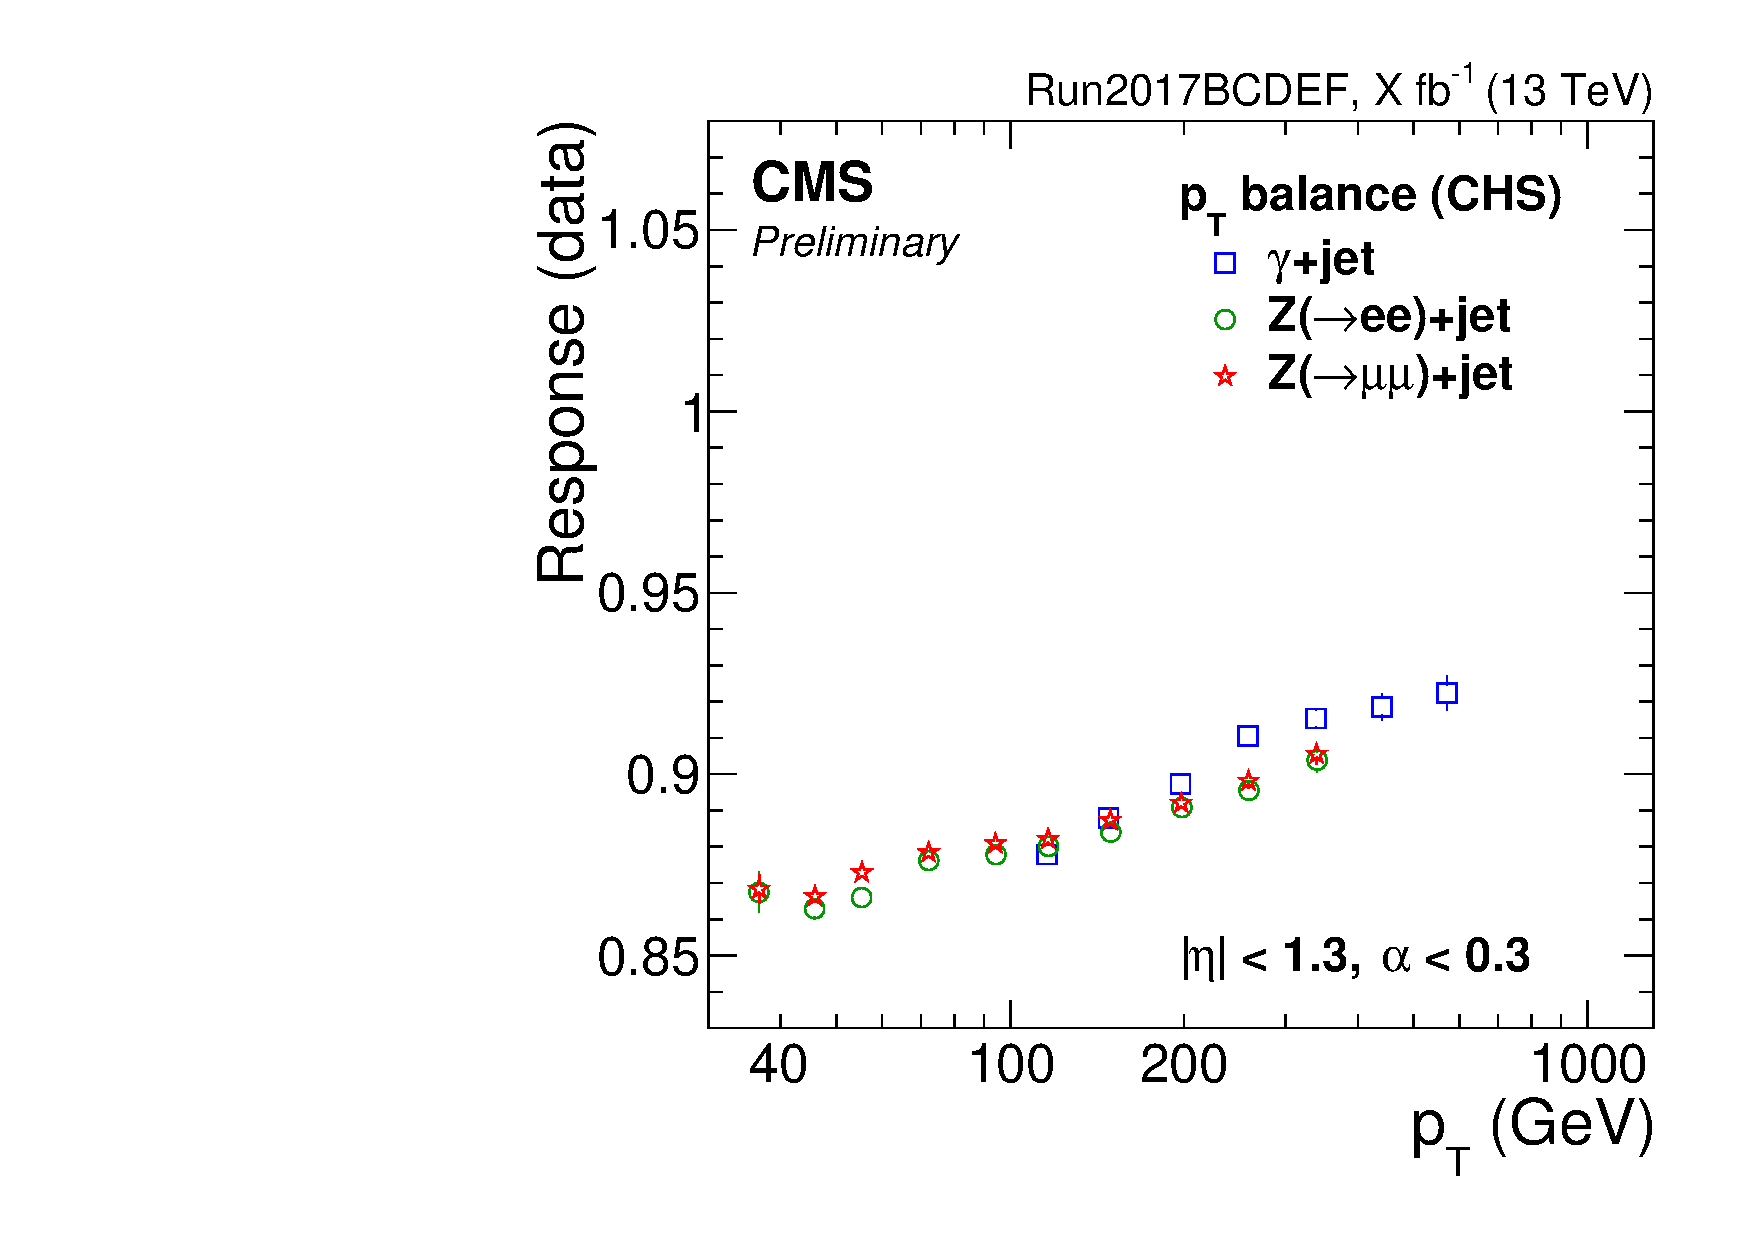
\includegraphics[width=0.10\textwidth]{BCDEFGH/paper_softrad_data_ptchs_vspt.pdf}
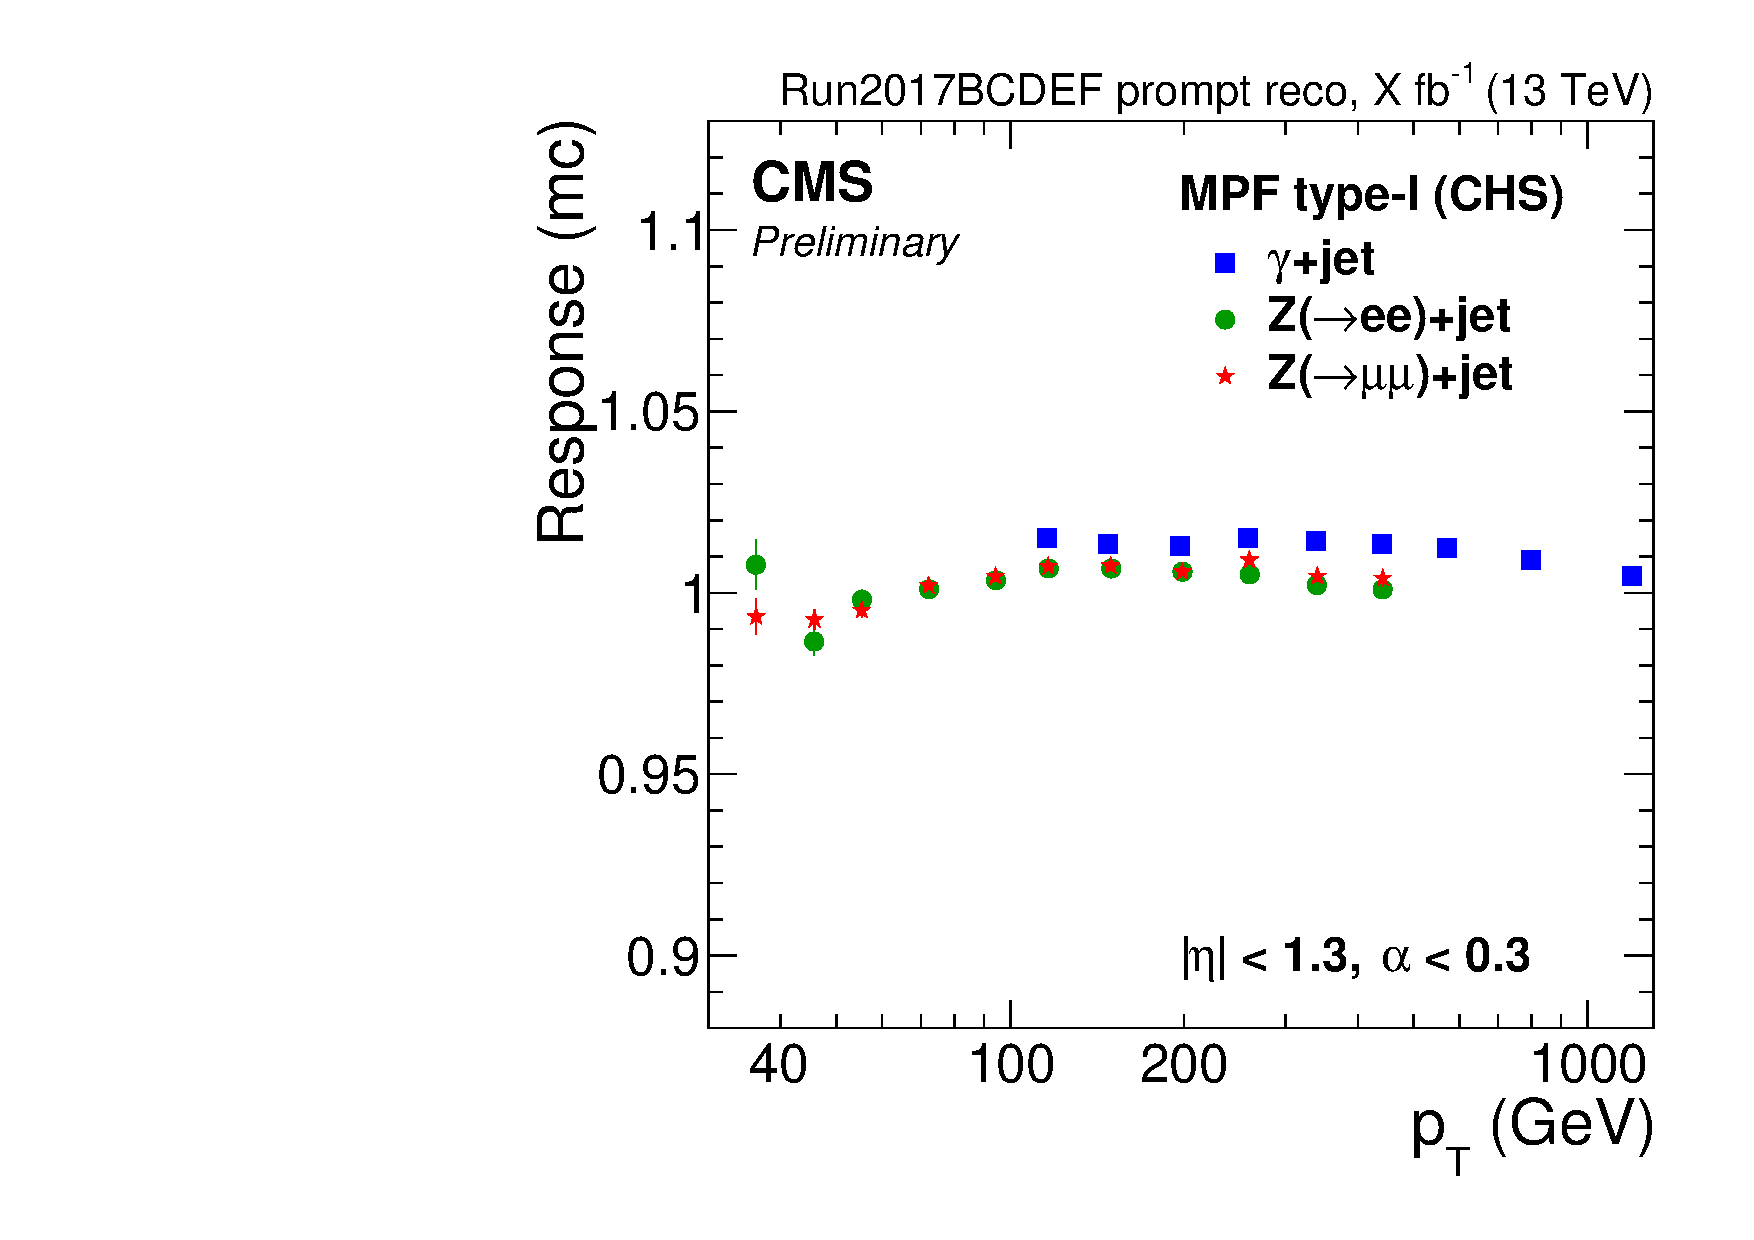
\includegraphics[width=0.10\textwidth]{BCDEFGH/paper_softrad_mc_mpfchs1_vspt.pdf}
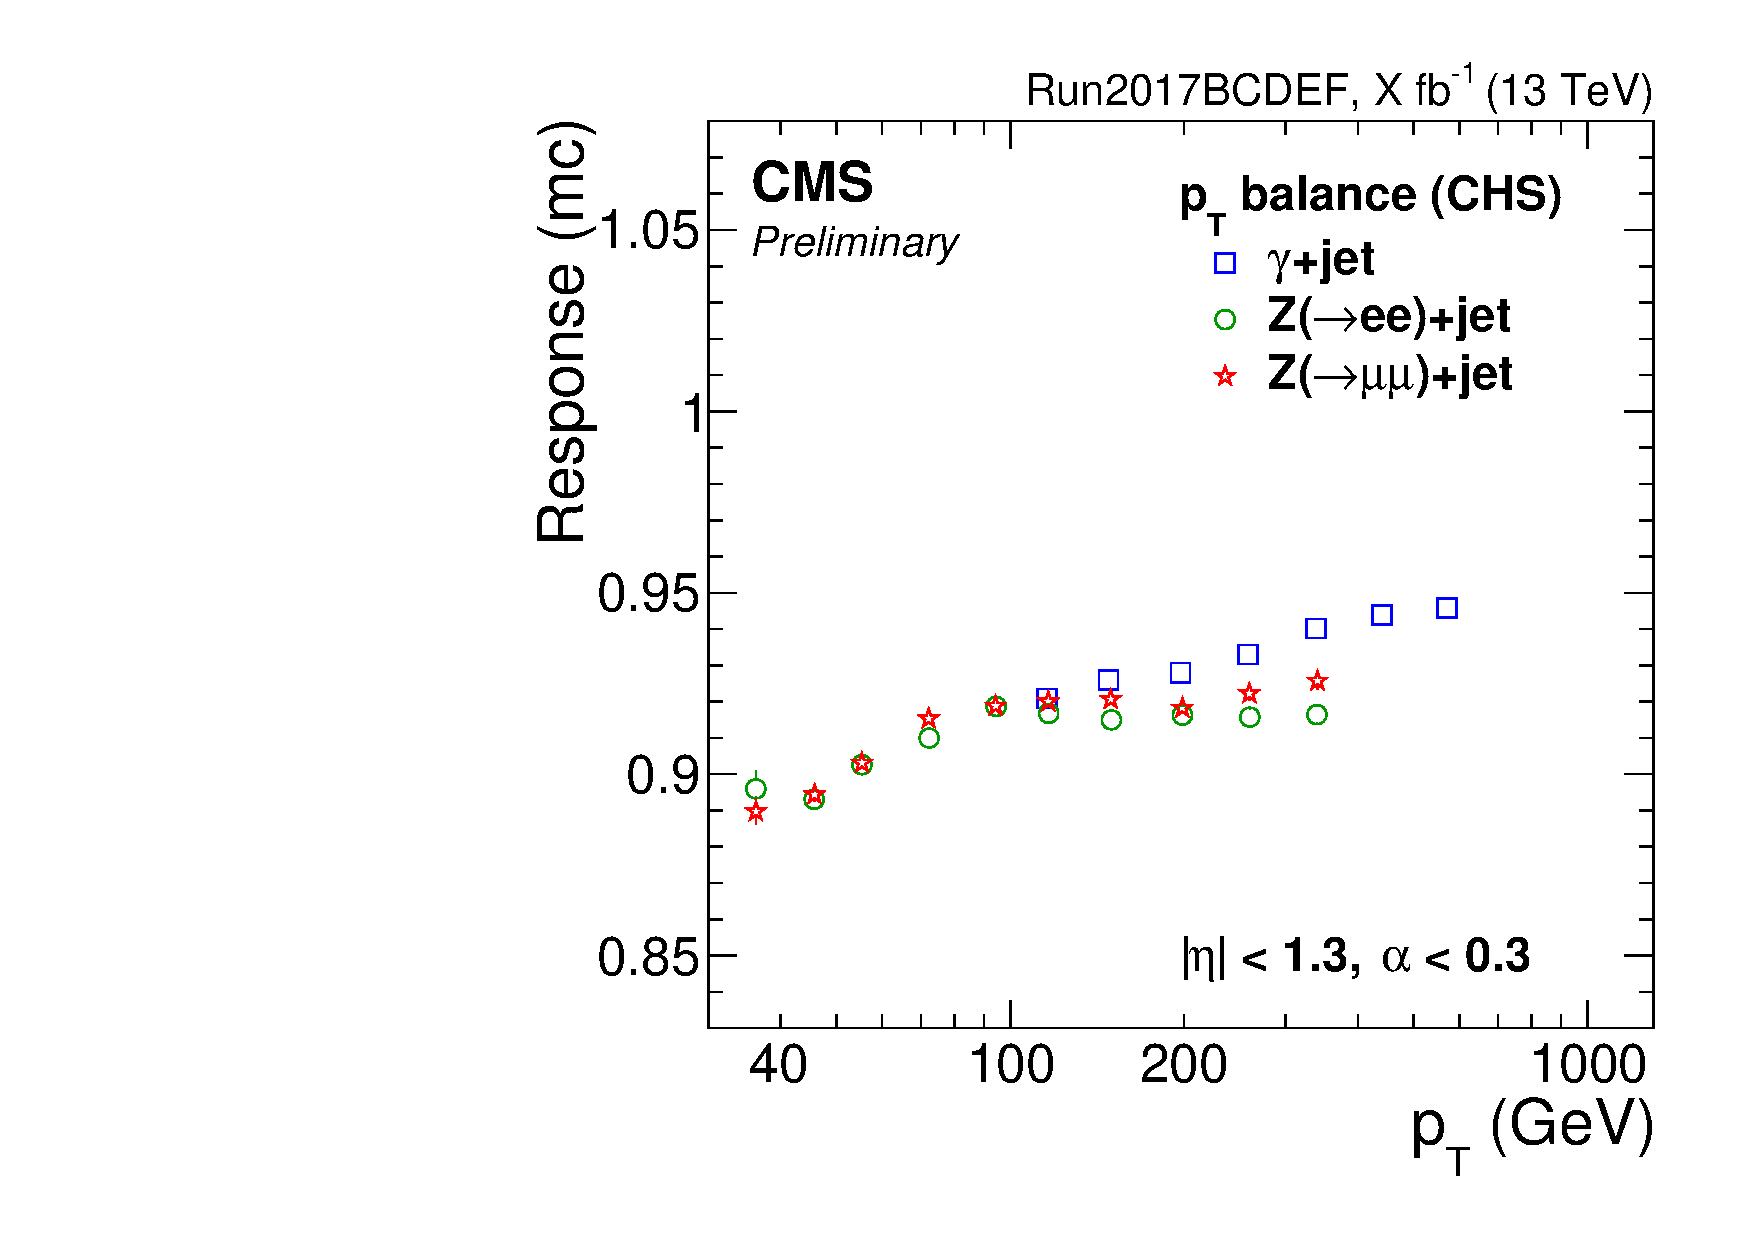
\includegraphics[width=0.10\textwidth]{BCDEFGH/paper_softrad_mc_ptchs_vspt.pdf}
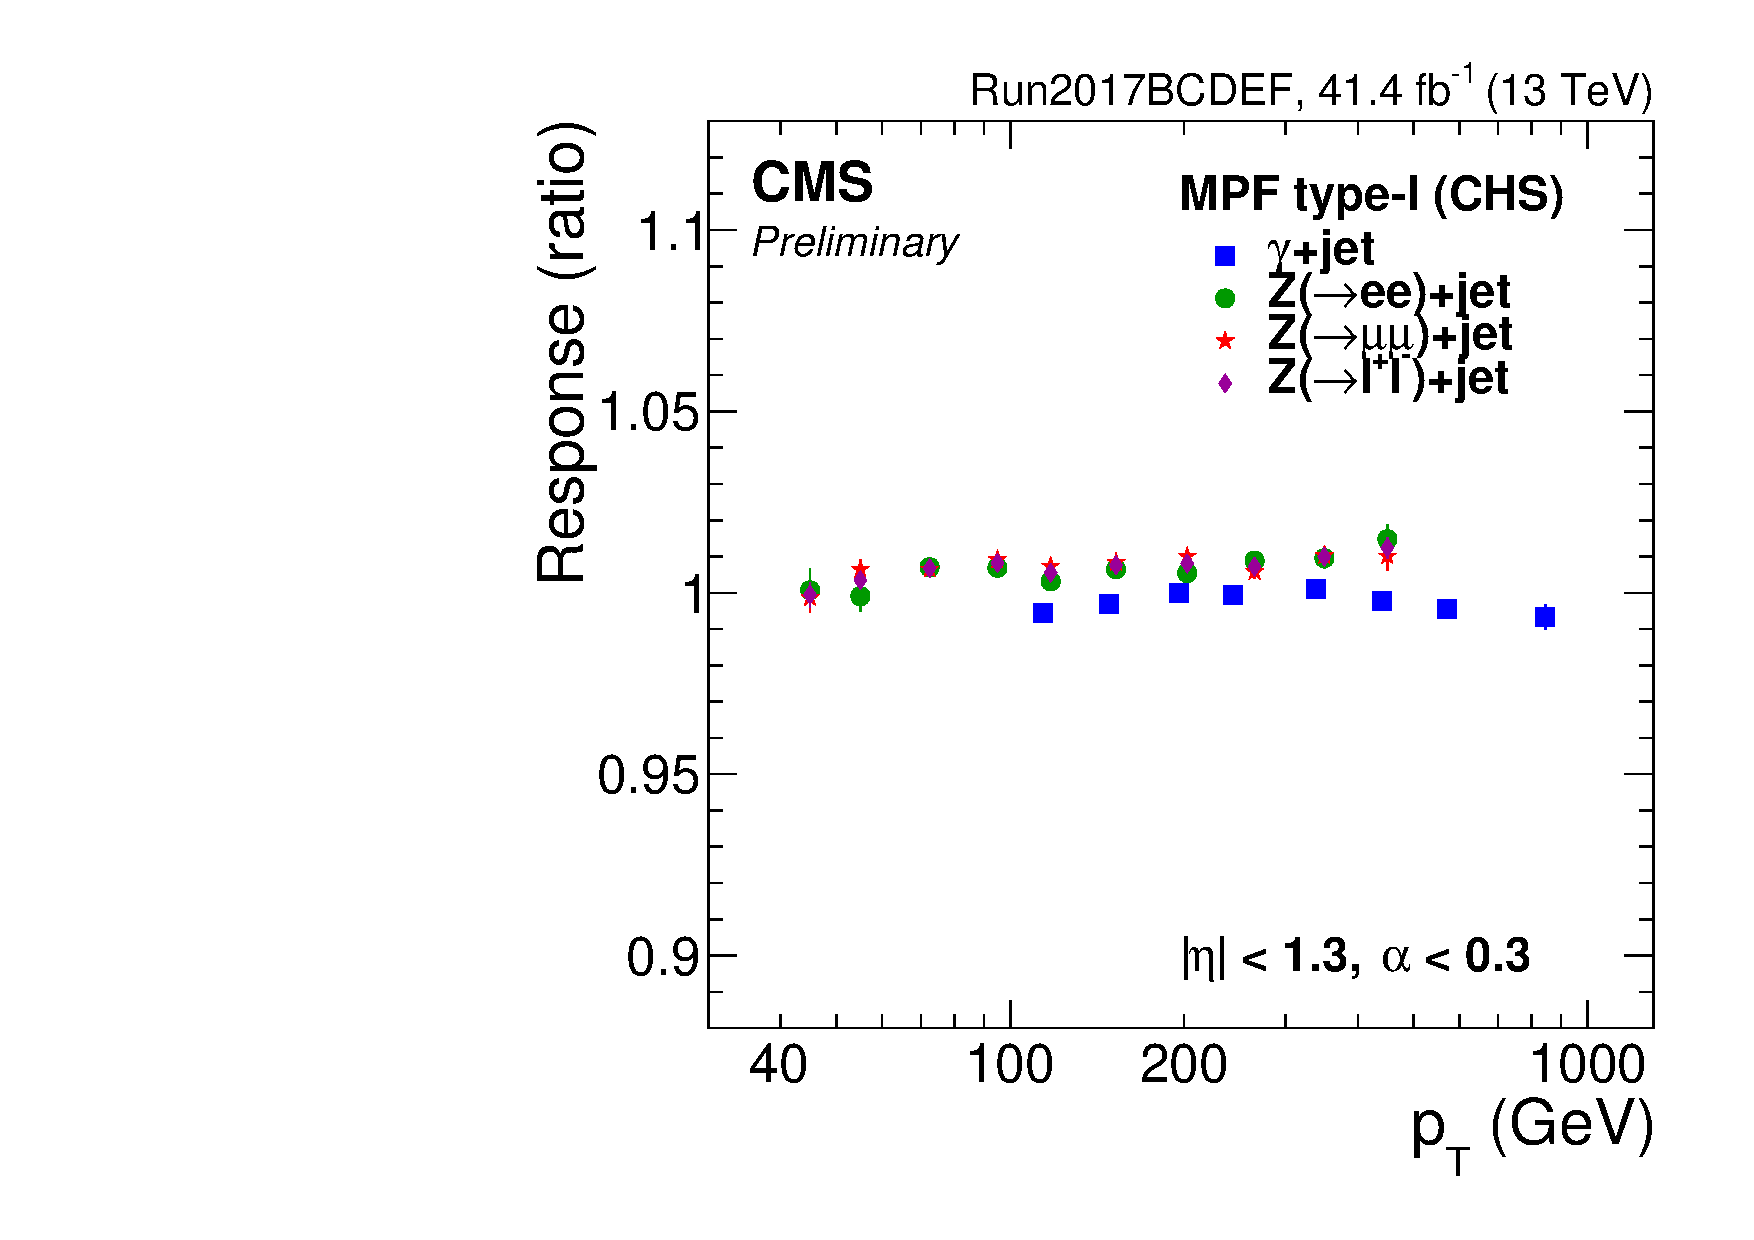
\includegraphics[width=0.10\textwidth]{BCDEFGH/paper_softrad_ratio_mpfchs1_vspt.pdf}
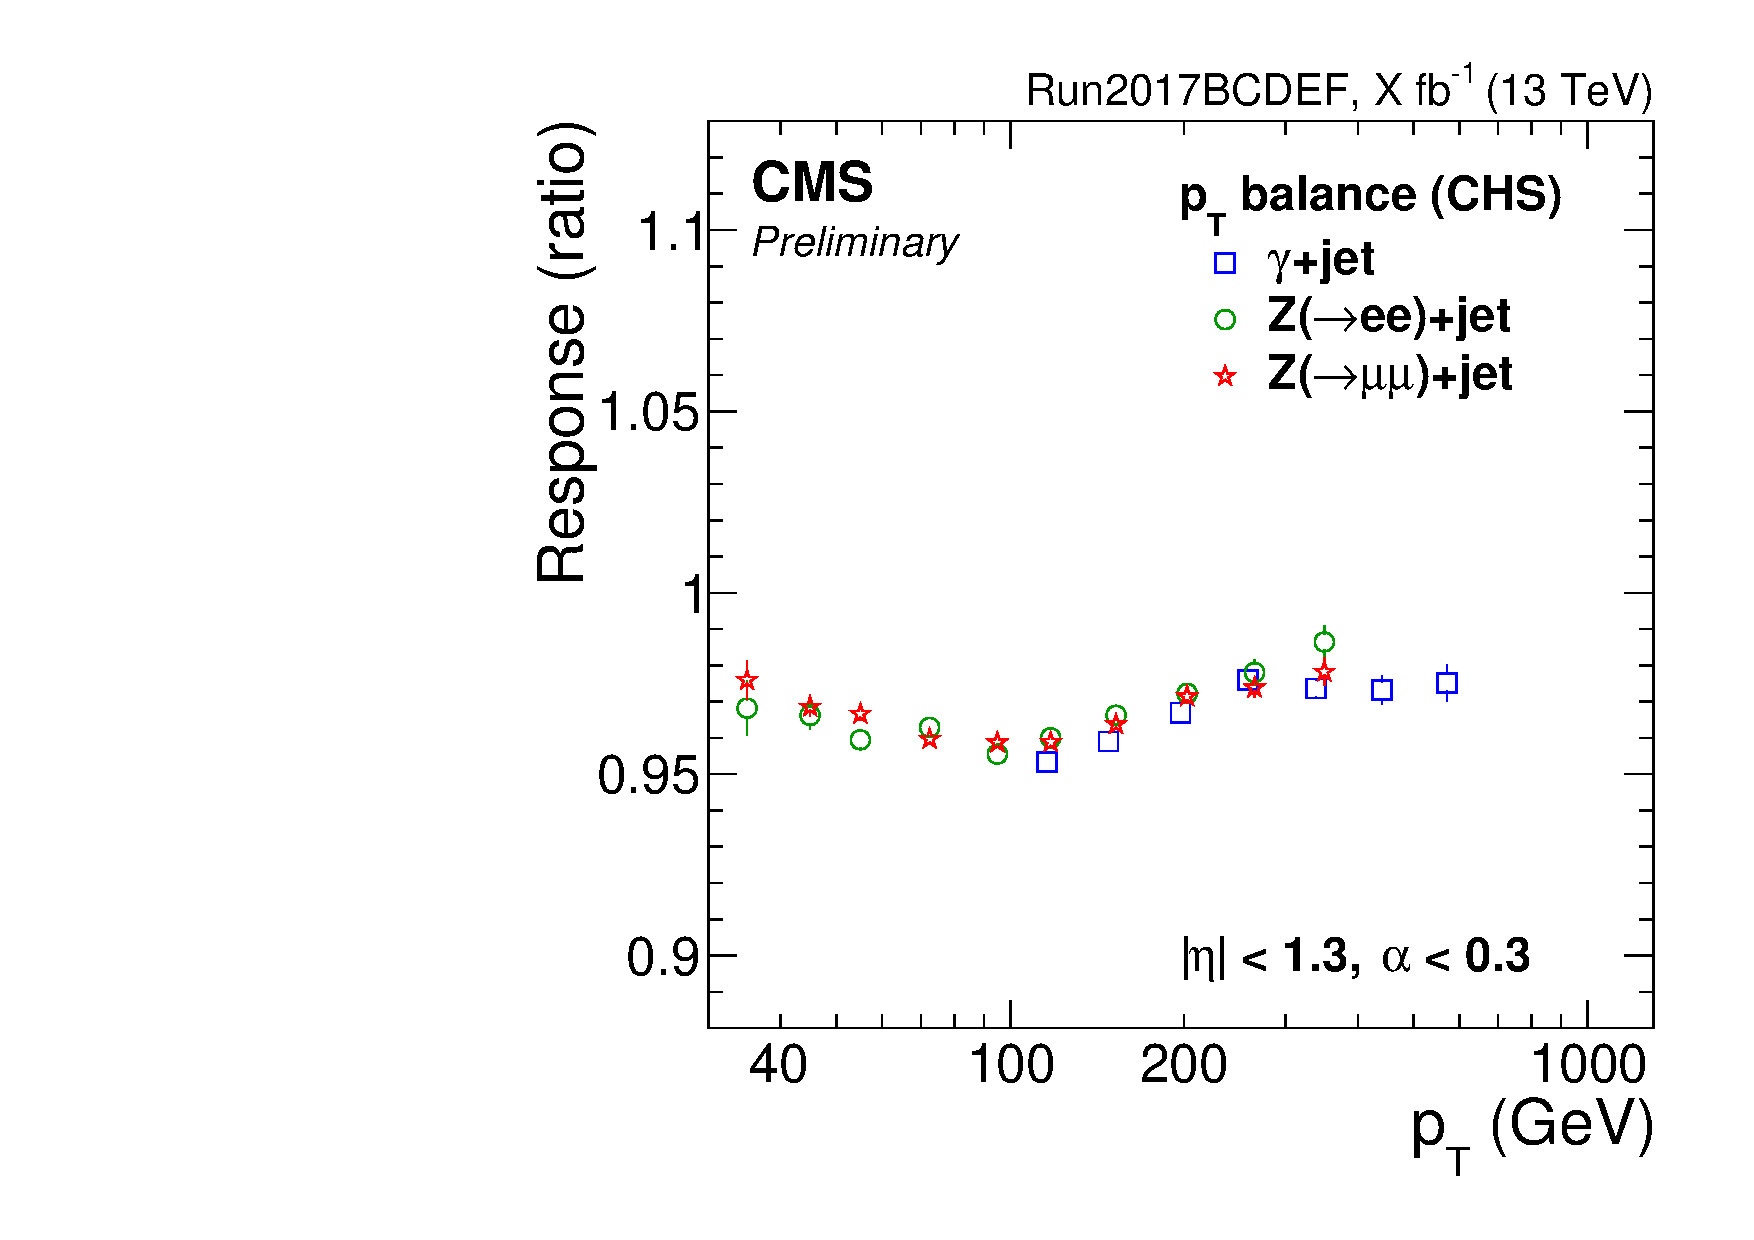
\includegraphics[width=0.10\textwidth]{BCDEFGH/paper_softrad_ratio_ptchs_vspt.pdf}



\foreach \n in \FineEtaBins{
  \newpage
%  \n \\
  \includegraphics[width=0.32\textwidth]{BCDEFGH/globalFitL3res_raw\n.pdf}
  \includegraphics[width=0.32\textwidth]{BCDEFGH/globalFitL3res_orig\n.pdf}
  \includegraphics[width=0.32\textwidth]{BCDEFGH/globalFitL3res_shifted\n.pdf}\\
  \includegraphics[width=0.30\textwidth]{BCDEFGH/softrad_2x6_kfsr\n.pdf}
  \includegraphics[width=0.30\textwidth]{BCDEFGH/softrad_2x6_vspt\n.pdf}
  \includegraphics[width=0.20\textwidth]{BCDEFGH/softrad_3x3_ratio_mpfchs1_vsalpha\n.pdf}
  \includegraphics[width=0.20\textwidth]{BCDEFGH/softrad_3x3_ratio_ptchs_vsalpha\n.pdf}\\

  \includegraphics[width=0.15\textwidth]{BCDEFGH/softrad_3x3_data_mpfchs1_vsalpha\n.pdf}
  \includegraphics[width=0.15\textwidth]{BCDEFGH/softrad_3x3_data_ptchs_vsalpha\n.pdf}
  \includegraphics[width=0.15\textwidth]{BCDEFGH/softrad_3x3_mc_mpfchs1_vsalpha\n.pdf} 
  \includegraphics[width=0.15\textwidth]{BCDEFGH/softrad_3x3_mc_ptchs_vsalpha\n.pdf}  
  \includegraphics[width=0.10\textwidth]{BCDEFGH/globalFitL3res_hsrc\n.pdf}
  \includegraphics[width=0.10\textwidth]{BCDEFGH/globalFitL3res_mpfchs1_kfsr\n.pdf}
  \includegraphics[width=0.10\textwidth]{BCDEFGH/globalFitL3res_ptchs_kfsr\n.pdf}\\

  \includegraphics[width=0.10\textwidth]{BCDEFGH/an_softrad_data_mpfchs1\n_vspt.pdf}
  \includegraphics[width=0.10\textwidth]{BCDEFGH/an_softrad_data_ptchs\n_vspt.pdf}
  \includegraphics[width=0.10\textwidth]{BCDEFGH/an_softrad_mc_mpfchs1\n_vspt.pdf}
  \includegraphics[width=0.10\textwidth]{BCDEFGH/an_softrad_mc_ptchs\n_vspt.pdf}
  \includegraphics[width=0.10\textwidth]{BCDEFGH/an_softrad_ratio_mpfchs1\n_vspt.pdf}
  \includegraphics[width=0.10\textwidth]{BCDEFGH/an_softrad_ratio_ptchs\n_vspt.pdf}


}


\newpage


\end{document}
